\documentclass[conference]{IEEEtran}
\IEEEoverridecommandlockouts
% The preceding line is only needed to identify funding in the first footnote. If that is unneeded, please comment it out.
\usepackage{cite}
\usepackage{amsmath,amssymb,amsfonts}
\usepackage{algorithmic}
\usepackage{graphicx}
\usepackage{textcomp}
\usepackage{xcolor}
\usepackage[brazilian]{babel}
\def\BibTeX{{\rm B\kern-.05em{\sc i\kern-.025em b}\kern-.08em
    T\kern-.1667em\lower.7ex\hbox{E}\kern-.125emX}}
\begin{document}

\title{Homework 1 - Alternativa 1\\
{\footnotesize \textsuperscript{*}Obs1: Todo o código utilizado neste relatório foi disponibilizado publicamente no repositório https://github.com/Glautor/Homework1-ICA-UFC}
}

\author{\IEEEauthorblockN{1\textsuperscript{o} Ramiro de Castro}
\IEEEauthorblockA{
\textit{Universidade Federal do Ceará (UFC)}\\
Fortaleza, Brasil \\
ramirorrccastro@gmail.com}
\and
\IEEEauthorblockN{2\textsuperscript{o} Glauton Santos}
\IEEEauthorblockA{
\textit{Universidade Federal do Ceará (UFC)}\\
Fortaleza, Brasil \\
glautoncardoso@gmail.com}
\and
\IEEEauthorblockN{3\textsuperscript{o} Gustavo Fechine}
\IEEEauthorblockA{
\textit{Universidade Federal do Ceará (UFC)}\\
Fortaleza, Brasil \\
gustavofechine@gmail.com}
}

\maketitle

\begin{abstract}
Este artigo é voltado à apresentar técnicas de pré-processamento 
de dados pegando como referência o dataset de B. German, "Glass Identification".
A partir do tratamento desses dados, é possível analizar com mais clareza as relações 
entre as características dos vidros e seus respectivos tipos.
\end{abstract}

\section{Introdução}
Vidros são de grande importância na ciência forense, tendo em vista as valiosas informações referentes a sua estrutura. 
A partir de pequenos fragmentos é possível identificar sua composição elementar e seu índice de refração, o que permite examinar
os frequentes fragmentos de vidro encontrados nas roupas de suspeitos de crimes como arrombamentos de casas.
Daí vem a necessidade do tratamento de dados referentes a composição dos vidros, sendo que, a partir disso, é possível determinar as 
possíveis origens desses fragmentos.
O presente trabalho se dipôs a analisar o pré-processamento dos dados do dataset "Glass Identification" de B. German, com o intuito de facilitar a compreensão das relações existentes
entre os dados, tais como as características constituintes do vidro (variáveis) se relacionam com os tipos de cada vidro (classes). 

\section{Metodologia}

Utilizando o dataset de Vidros, o qual foi obtido do repositório de Machine Learning da UCI[4], procurou-se entender como sua estrutura funciona. Neste conjunto de dados, 
existem 10 variáveis independentes (preditores): 1.RI: Índice Refrativo, 2. Na: Sódio, 3. Mg: Magnésio, 4. Al: Alumínio, 5. Si: Silício, 6. K: Potássio, 7. Ca: Cálcio , 8. Ba: Bário, 
9. Fe: Ferro, 10. Type: Tipo de vidro. As variáveis 2 a 9 estão medidas na porcentagem de peso em que cada um de seus óxidos está presente no vidro, e a variável Tipo classifica
as amostrar de vidro em 7 tipos: 1. Vidro de Construção Flutuante Processado , 2. Vidro de Construção Não Flutuante Processado ,
3.Vidro de Carro Flutuante Processado, 4. Vidro de Carro Não Flutuante Processado (não está presente no dataset), 5. Vidro de Containeres, 6. Vidro de Copo, 7. Vidro de Farol.

Conhecendo as variáveis do dataset, uso-se da linguagem R[2] e dos seguintes pacotes: corrplot[6], factorextra[6], ggplot2[3], e executou-se os seguintes procedimentos:

2.1 Análise Monovariada e Não-Condicional dos Dados
	Primeiramente, calculou-se a média, desvio padrão, e skewness (simetria) de cada um dos preditores e então foi feita uma tabela (Tabela 1) com os valors encontrados.
	Cada uma dessas medidas tem a sua devida importância no entendimento dos dados, a média fornece o valor com a maior probabilidade de ser encontrado nas amostras (Valor Esperado),
	o desvio padrão mostra a dispersão dos dados em relação a média, e a skewness mostra a simetria, ou falta dela, dos dados, uma skewness positiva indica que os dados estão mais deslocados
	para a direta da média, e uma skewness negativa indica que os dados estão deslocados para a esquerda da média.
	Por fim, foram plotados os histogramas de cada um dos preditores, sendo possível conferir visualmente a representação das medidas anteriormente calculadas.
	Após anasilar estas informações, decidiu-se por mostrar os histogramas de Magnésio (Figura 1) e Calcio (Figura 3), pois estes apresentam os maiores desvio padrão, e o histograma de Potássio (Figura 2) , pois este apresenta a maior 
	assimetria (uma skewness bem maior que zero), o que pode significar a presença de outliers, que devem ser devidamente tratados.

2.2 Análise Monovariada e Classe-Condicional dos Dados
	Tendo sido feita uma análise geral dos dados, agora é feito uma análise por classe (tipo) de vidro, seguindo os mesmos passos do item anterior.
	Analisando esses dados, e pelos motivos do item anterior, selecionou-se para amostra os histogramas de Ca: Classe 2 (Figura 4), Potássio: Classe 5 (Figura 5),
	Potássio: Classe 7 (Figura 6), Magnésio: Classe 2 (Figura 7).
	

2.3 Análise Bivariada e Não-Condicional dos Dados
	Foi calculado a matriz de correlação das variáveis (Figura 8), e feito o gráfico de dispersão (scatterplot) para cada um dos pares. Analisando a matriz (Figura 9),
	e os gráficos gerados, foram considerados relevantes dois dos gráficos, o da relação Cálcio vs Índice Refracionário (Figura 8) e  Silício vs Índice Refracionário (Figura 8), onde o primeiro 
	apresenta uma correlação direta (0.84) e o segundo é inverso (-0.54).

2.4 Análise das Componetnes Principais
	A Análise das Componetnes Principais (PCA) foi feita utilizando-se de 2 Componentes Princiapais (PC), que juntas conseguem reprensentar uma variância de 53.5\% dos dados, como mostra a o gráfico
	de barras de variância por componente (Figura 10), e plotou-se o gráfico de dispersão destes dois PCs (Figura 11), onde as classes são as diferentes cores de pontos. 
	Esta análise é importante para poder-se analisar os dados diminuindo o número de preditores a serem analisados, e isto é feito com uma transformação ortogonal do plano dos dados orginais para
	um plano onde os eixos são os PCs selecionados.


\section{Resultados}
3.1 Propriedades Físico-Químicas Amostradas
	Olhando-se os histogramas condicionados pelas classes, é possível perceber a existência de outliers, na porcentagem de Bário, em várias classes [5], como pode ser visto
	na Figura X, em especial nas classes 2 e 5, onde há amostras cuja porcentagem de Bário está muito acima das demais.
	Analisando as amostras onde não existem porcentagem de K, Ba e Fe[5], é notável que das 14 ocorrências, todas as amostras da classe 6 estão presentes, e apenas uma amostra da classe 1
	está presente, e esta possui preditores bem diferentes dos achados na medidas calculadas para sua classe, o que indica que possivelmente há amostras que podem ter sido classificadas incorretamente
	Uma outra análise interessante das propriedades dos tipos de vidros é a existência de Magnésio[5] nos tipos de vidro, apenas as classe 1 e 3 o possuem em sua composição.

3.2 O conjunto de Dados
	A falta da classe(tipo) 4 de vidro, e o excesso de amostras do tipo 1 e 2, quando comparado as amostras do tipo 3, 5, 6 e 7, faz com que naõ se tenha um grande grau de certeza
	para classificar um vidro como não residencial (que não seja tipo 1 ou 2), e não se sabe onde os outliers encontrados realmente pertençam, principalmente em relação ao vidro de tipo 4.
	Além disso, no PCA realizado, ficou evidente que mesmo que os 2 maiores componentes principais (PC) representem mais de 50\% da variância dos dados, como comentado na seção 2.4, é necessário
	usar mais PCs para que seja possível ter uma melhor compreensão dos dados.
	Para terminar, todos os códigos usados e gráficos gerados estão no link [5].

\begin{table}[h]
\centering
\caption{Média, Desvio Padrão e Simetria}
\vspace{0.5cm}
\begin{tabular}{r|r|r|r}
 
& Média & DP & Simetria \\
\hline
RI & 1.518 & 0.003 & 1.603 \\
Na & 13.408 & 0.817 & 0.448 \\
Mg & 2.685 & 1.442 & -1.136 \\
Al & 1.445 & 0.499 & 0.895 \\
Si & 72.651 & 0.775 & -0.720 \\
K & 0.497 & 0.652 & 6.460 \\
Ca & 8.957 & 1.423 & 2.018 \\
Ba & 0.175 & 0.497 & 3.369 \\
Fe & 0.057 & 0.097 & 1.730 \\
 
\end{tabular}
\end{table}

\newpage %% ou \clearpage

\begin{thebibliography}{00}
\bibitem{b1} R. Development Core Team, R: a language and environment for statistical computing, R Foundation for Statistical Computing, Vienna, Austria, ISBN: 3-900051-00-3, 2008, http://www.R-project.org.
\bibitem{b2} RStudio Team (2016). RStudio: Integrated Development for R. RStudio, Inc., Boston, MA, URL http://www.rstudio.com/.
\bibitem{b3} Wickham H (2016). ggplot2: Elegant Graphics for Data Analysis. Springer-Verlag New York. ISBN 978-3-319-24277-4, http://ggplot2.org.
\bibitem{b4} B. German. Central Research Establishment. Home Office Forensic Science Service. Aldermaston, Reading, Berkshire RG7 4PN. http://archive.ics.uci.edu/ml/datasets/Glass+Identification.
\bibitem{b5} Repositório aberto no github com o código utilizado neste relatório: https://github.com/Glautor/Homework1-ICA-UFC.
\bibitem{b6} R-Documentation. rdocumentation.org.
\end{thebibliography}
\vspace{12pt}

\newpage %% ou \clearpage
\section{Imagens de Referência - Questão 1}

\begin{figure}[h]
\caption{Histograma Mg}
\centering % para centralizarmos a figura
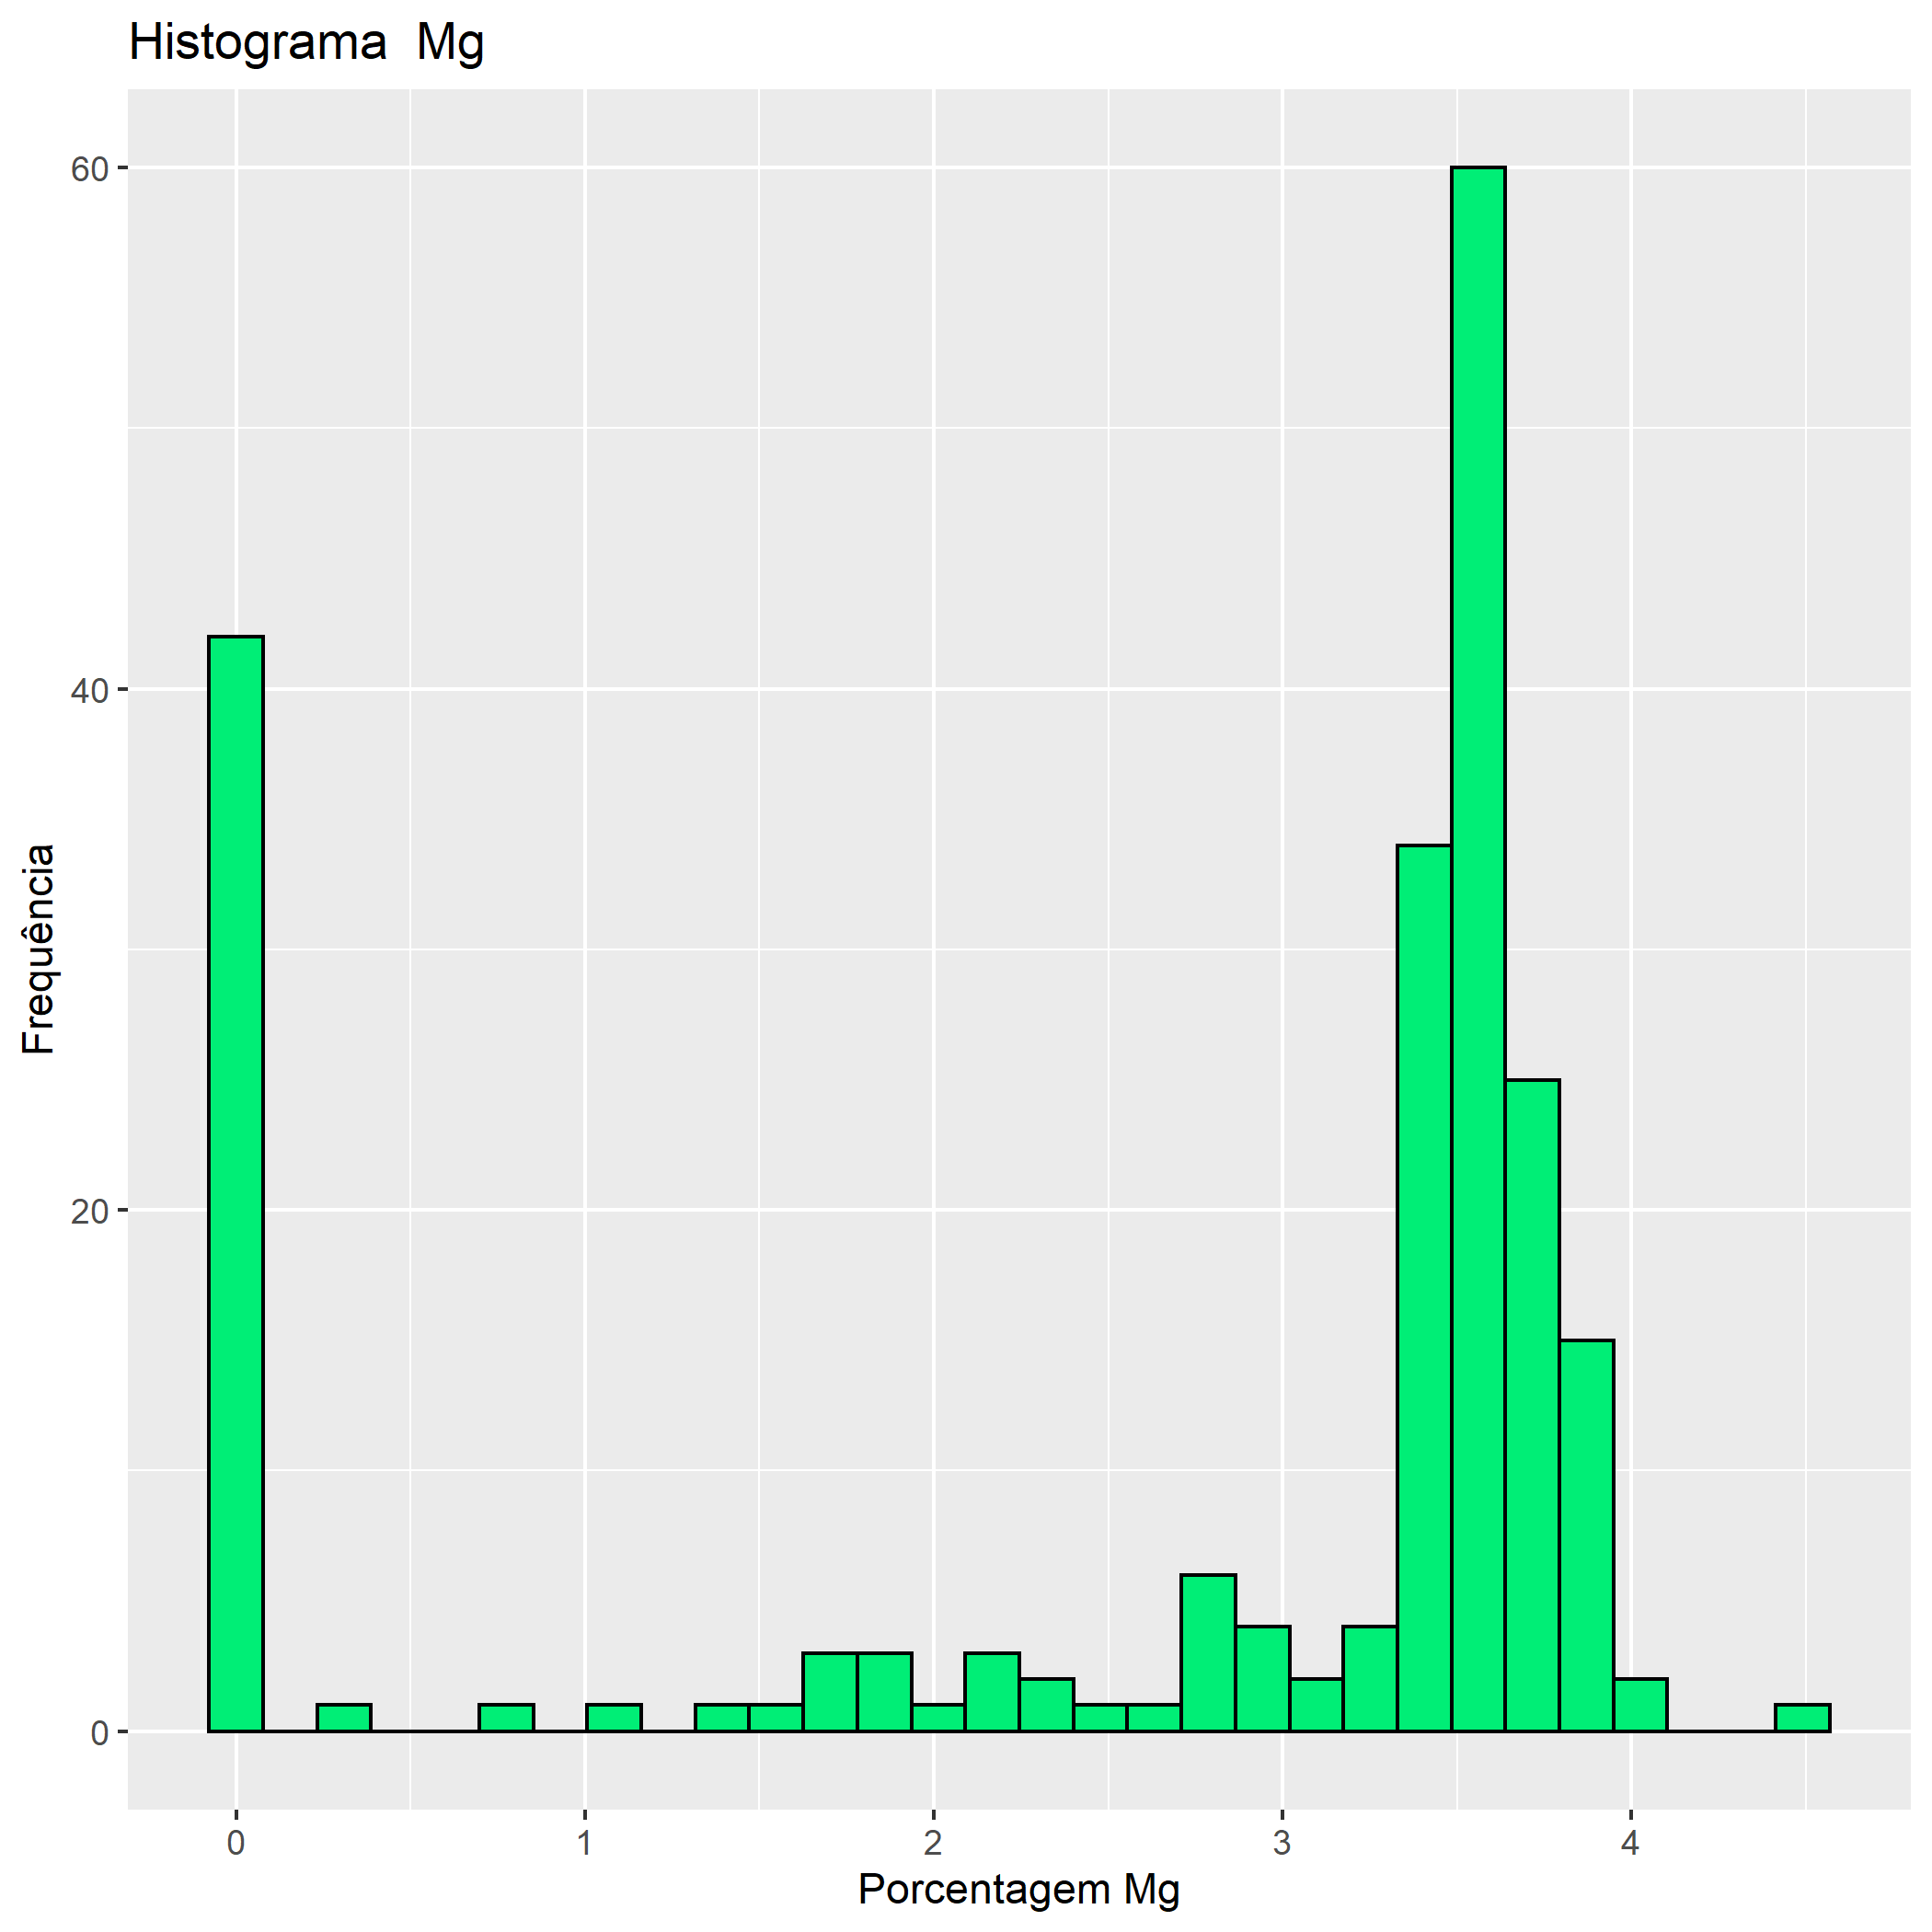
\includegraphics[width=5cm]{images/pt1/HistogramaMg.png} % leia abaixo
\label{figura:histogramaal}
\end{figure}



\begin{figure}[h]
\caption{Histograma K}
\centering % para centralizarmos a figura
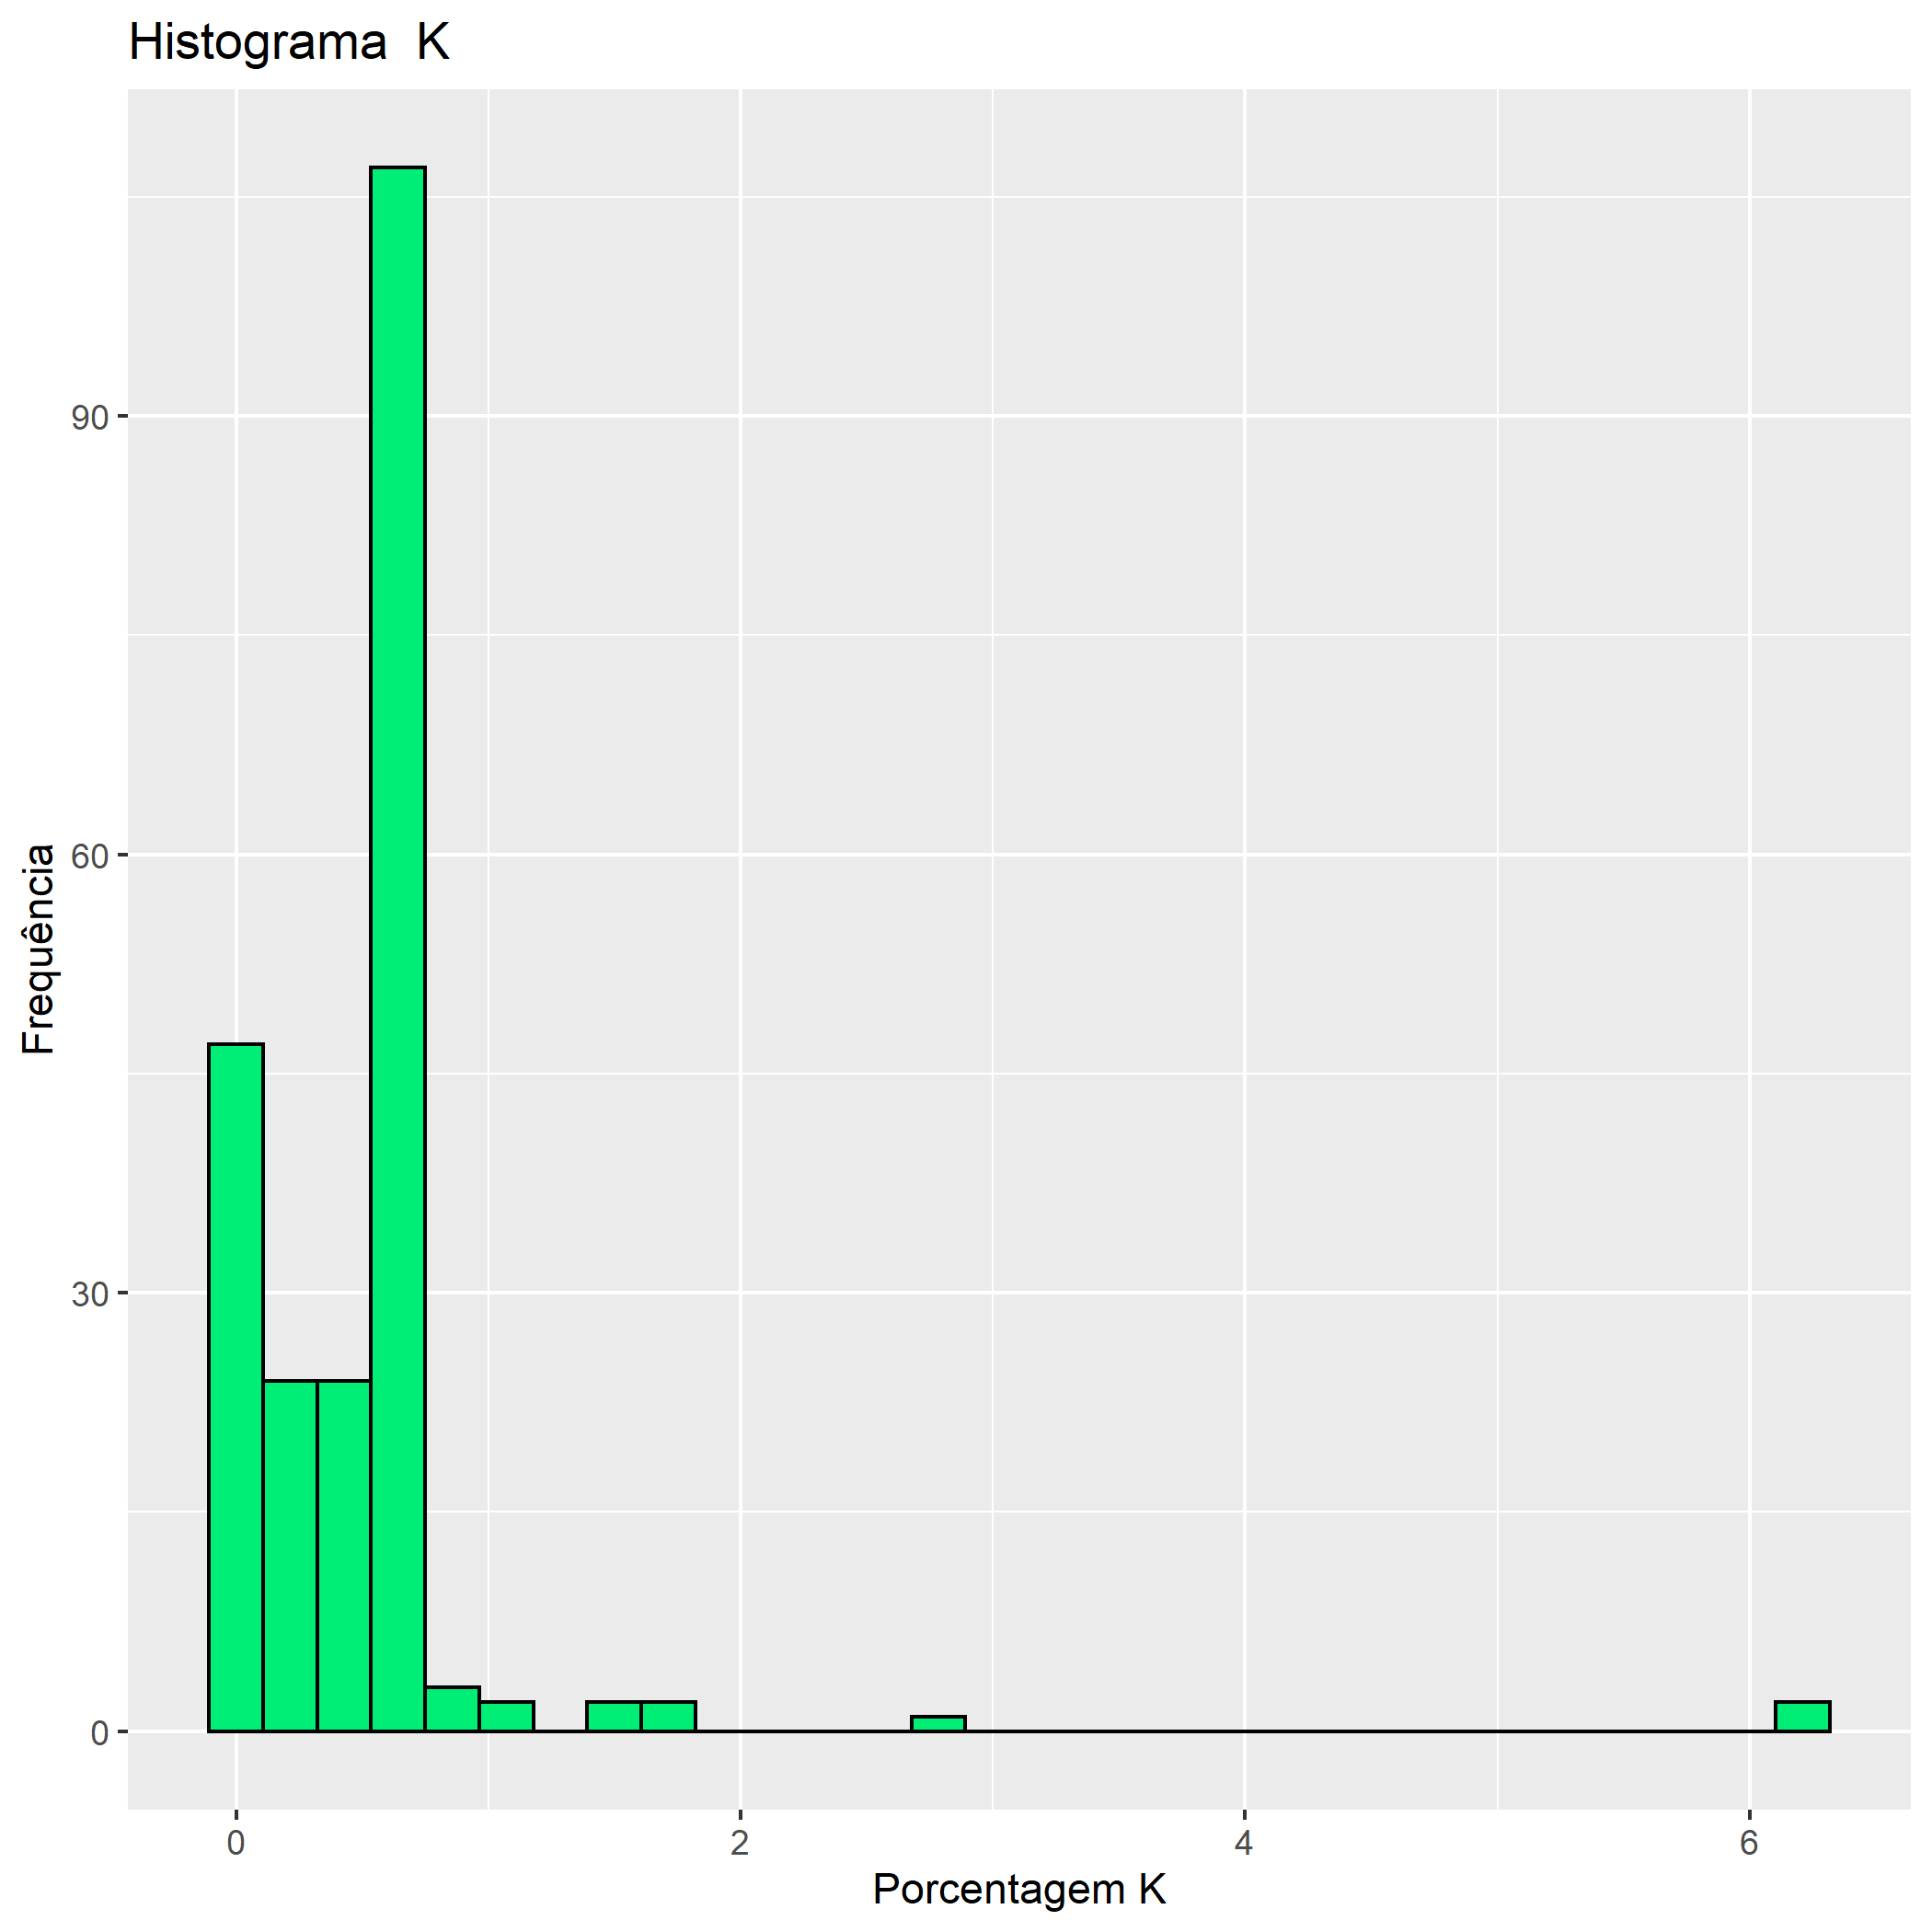
\includegraphics[width=5cm]{images/pt1/HistogramaK.png} % leia abaixo
\label{figura:histogramaal}
\end{figure}



\begin{figure}[h]
\caption{Histograma Ca}
\centering % para centralizarmos a figura
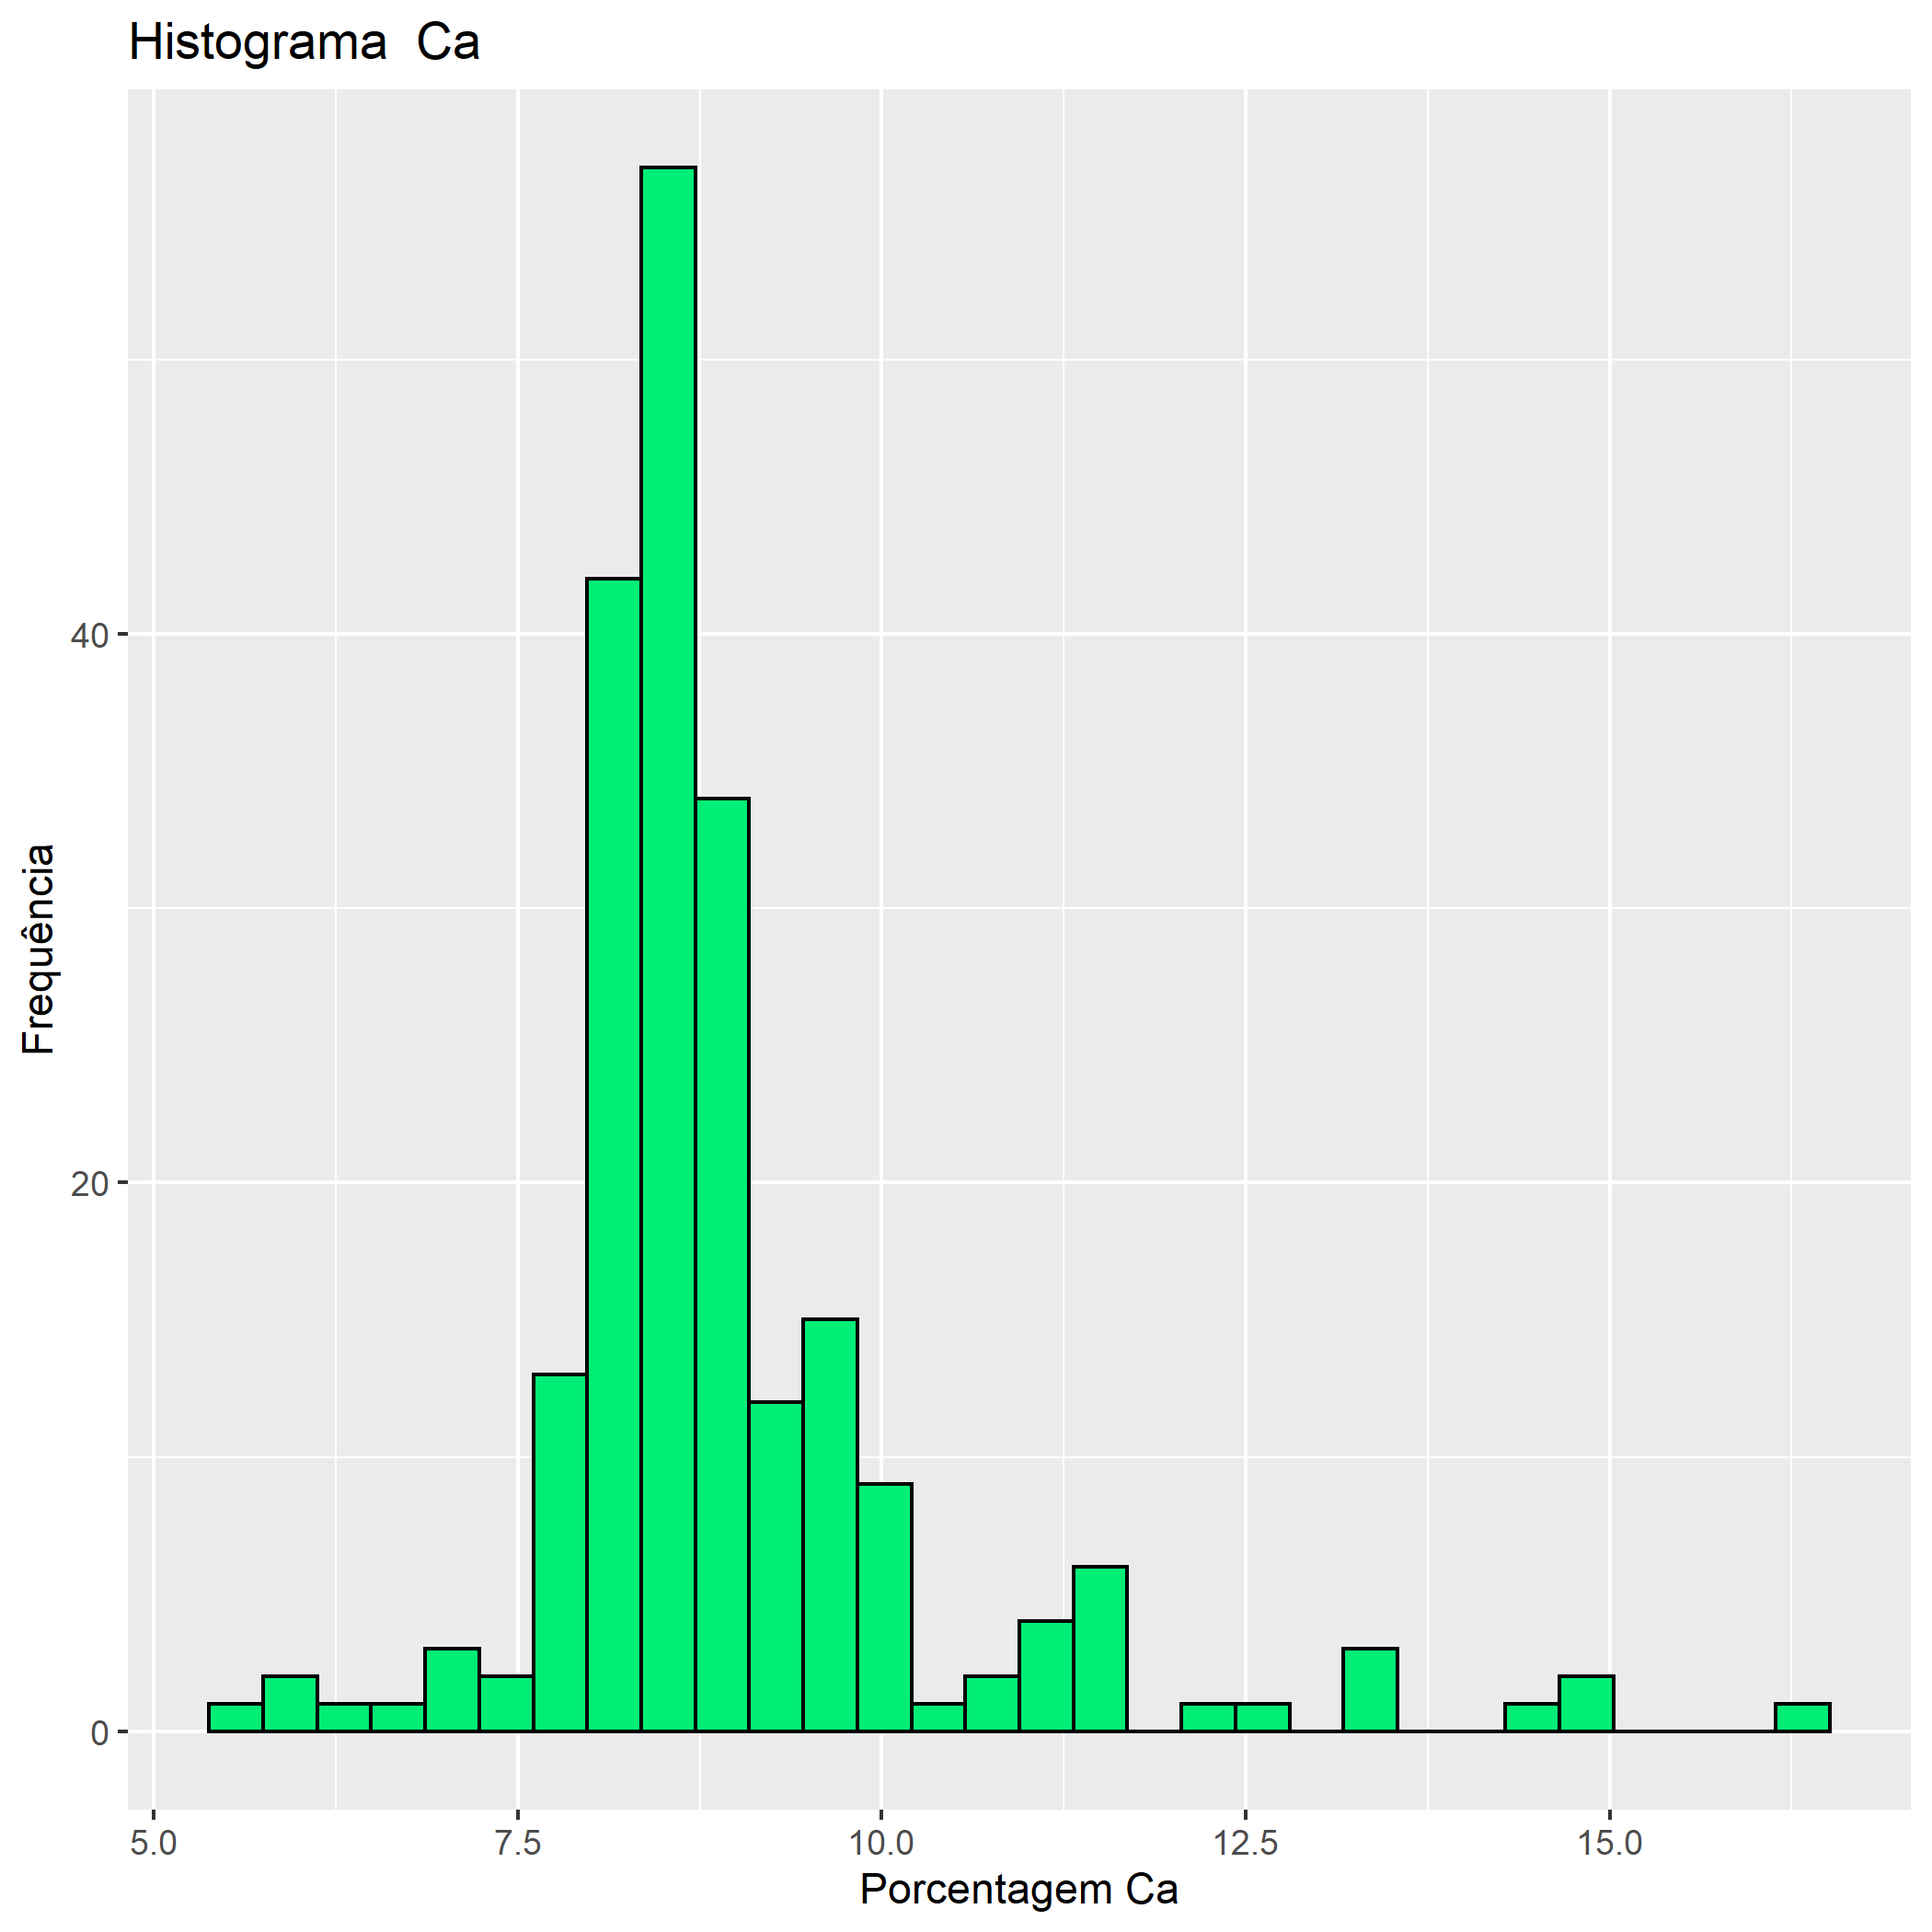
\includegraphics[width=5cm]{images/pt1/HistogramaCa.png} % leia abaixo
\label{figura:histogramaal}
\end{figure}


\newpage %% ou \clearpage
\section{Imagens de Referência - Questão 2}

\begin{figure}[h]
\caption{Histograma Ca - CLasse 2}
\centering % para centralizarmos a figura
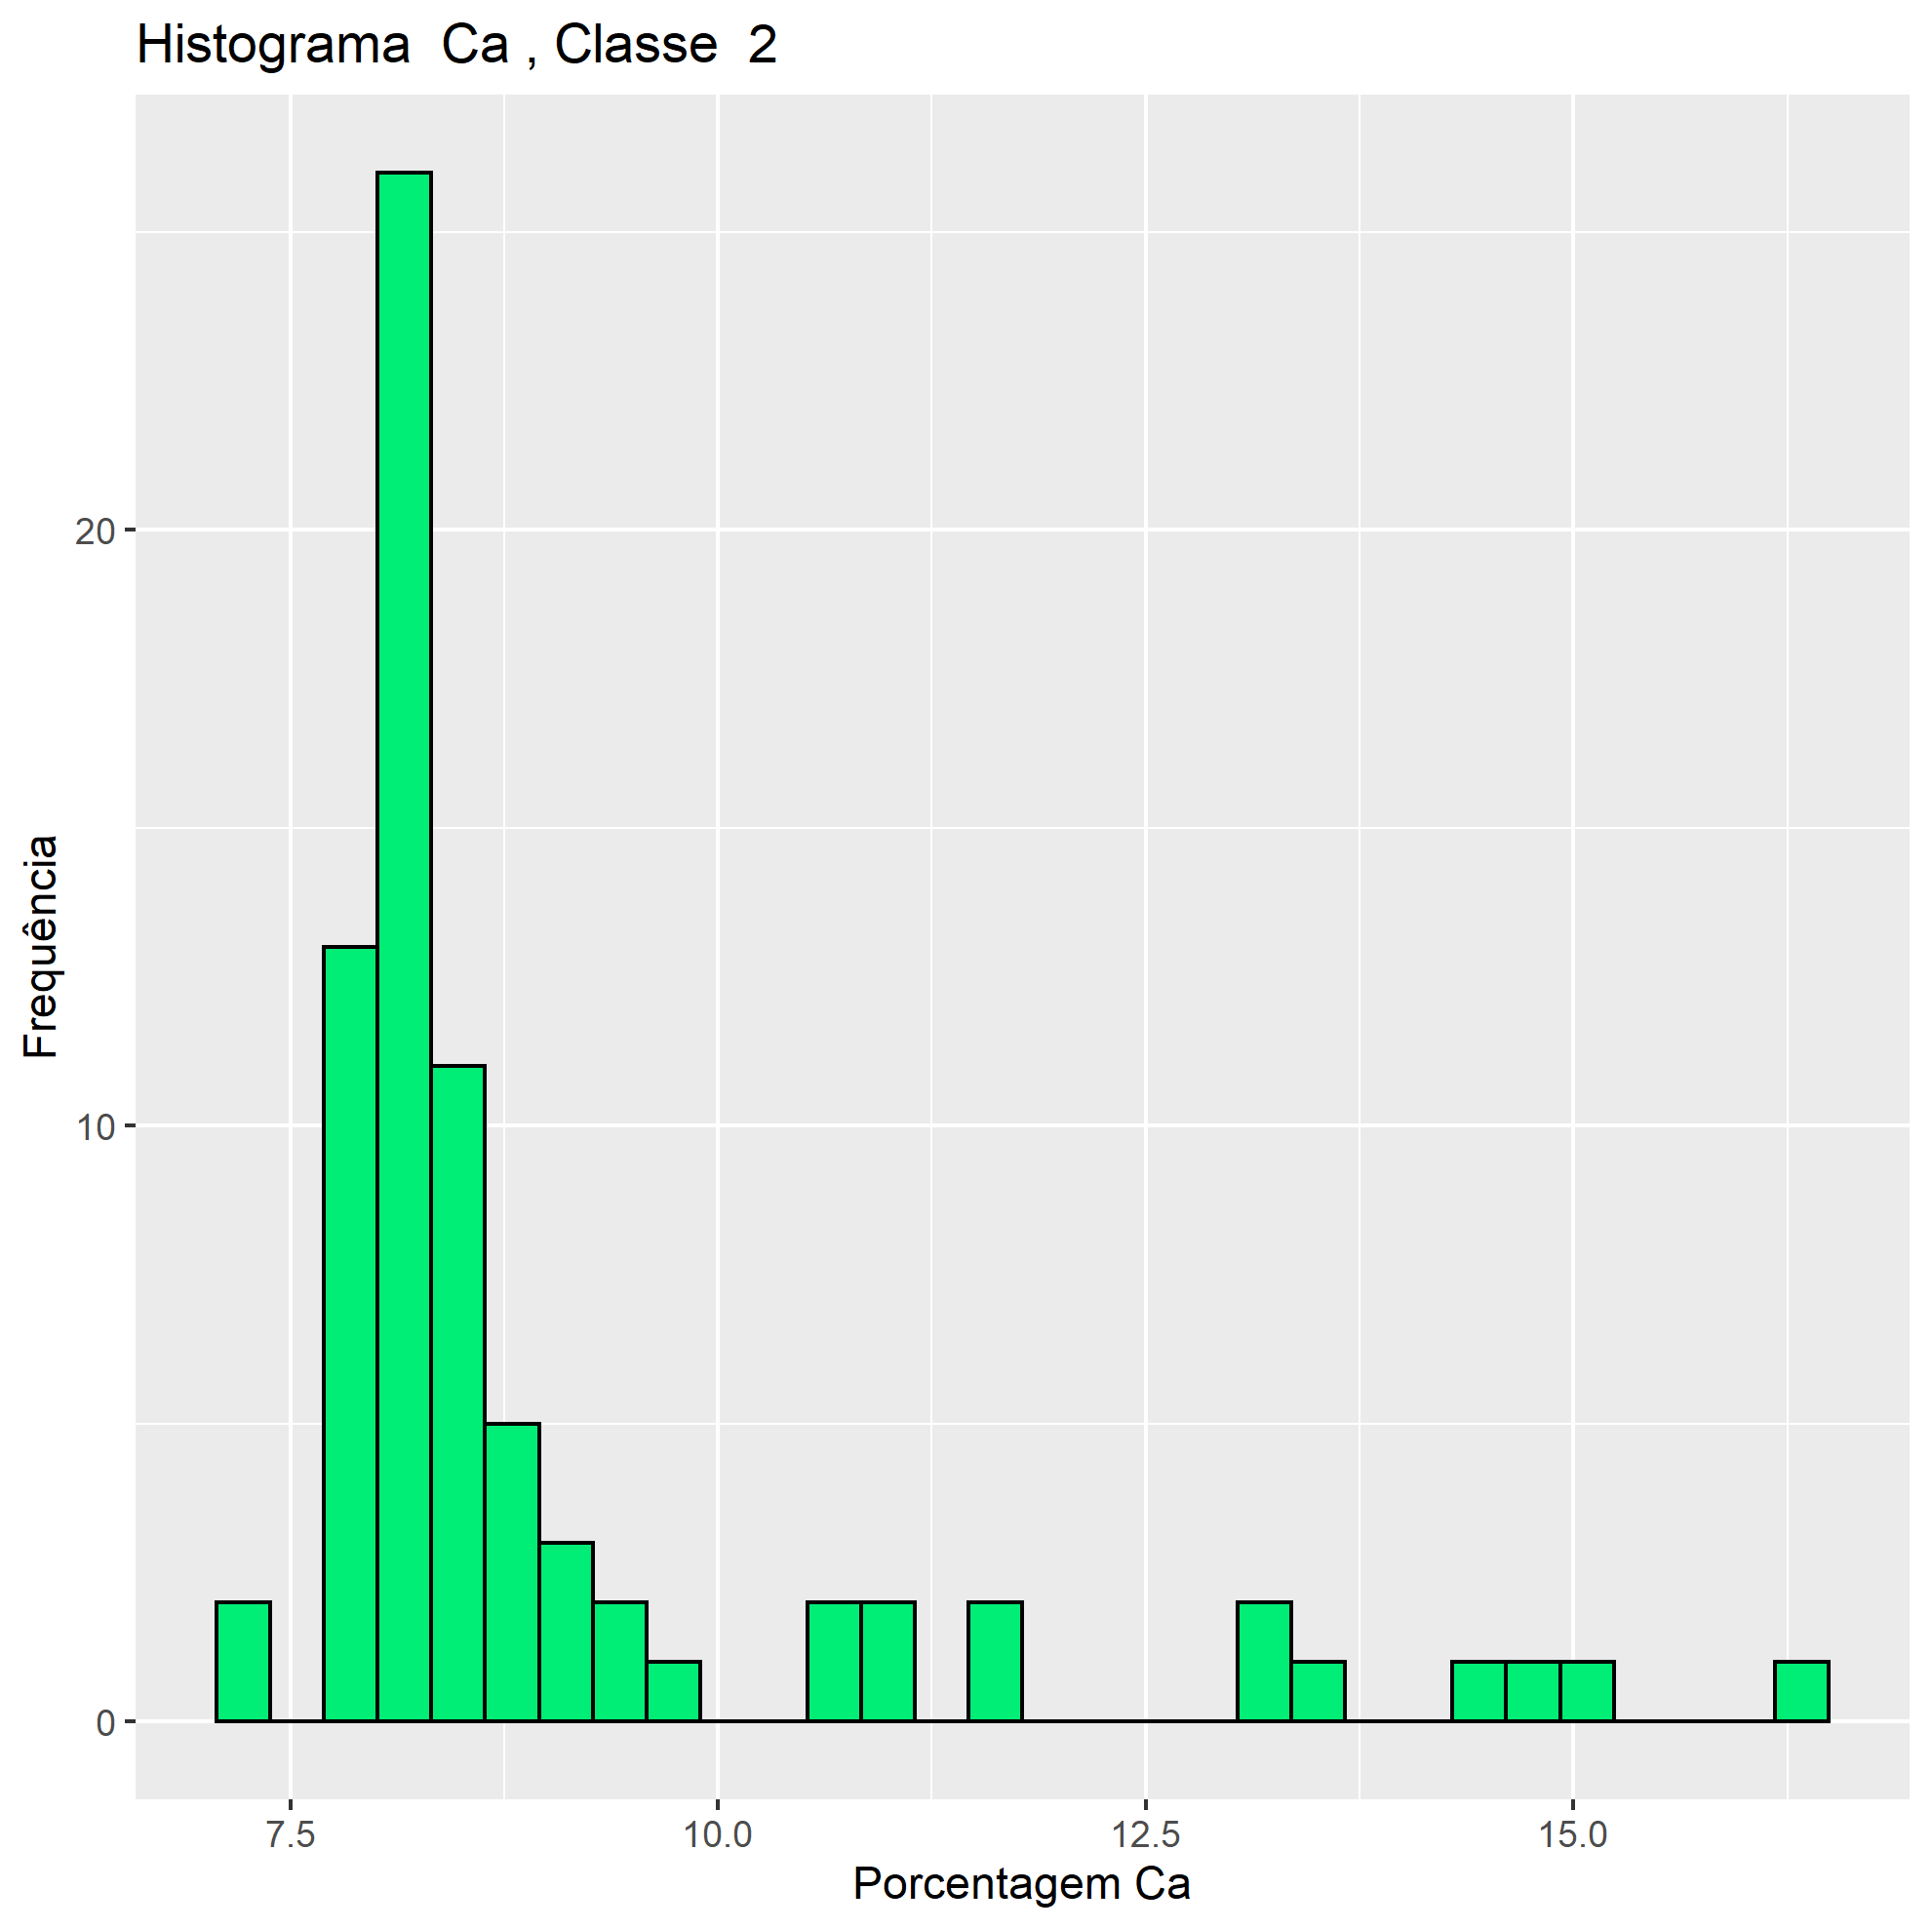
\includegraphics[width=5cm]{images/pt2/HistogramaCa_Classe2.png} % leia abaixo
\label{figura:histogramaal}
\end{figure}


\begin{figure}[h]
\caption{Histograma Ba - Classe 2}
\centering % para centralizarmos a figura
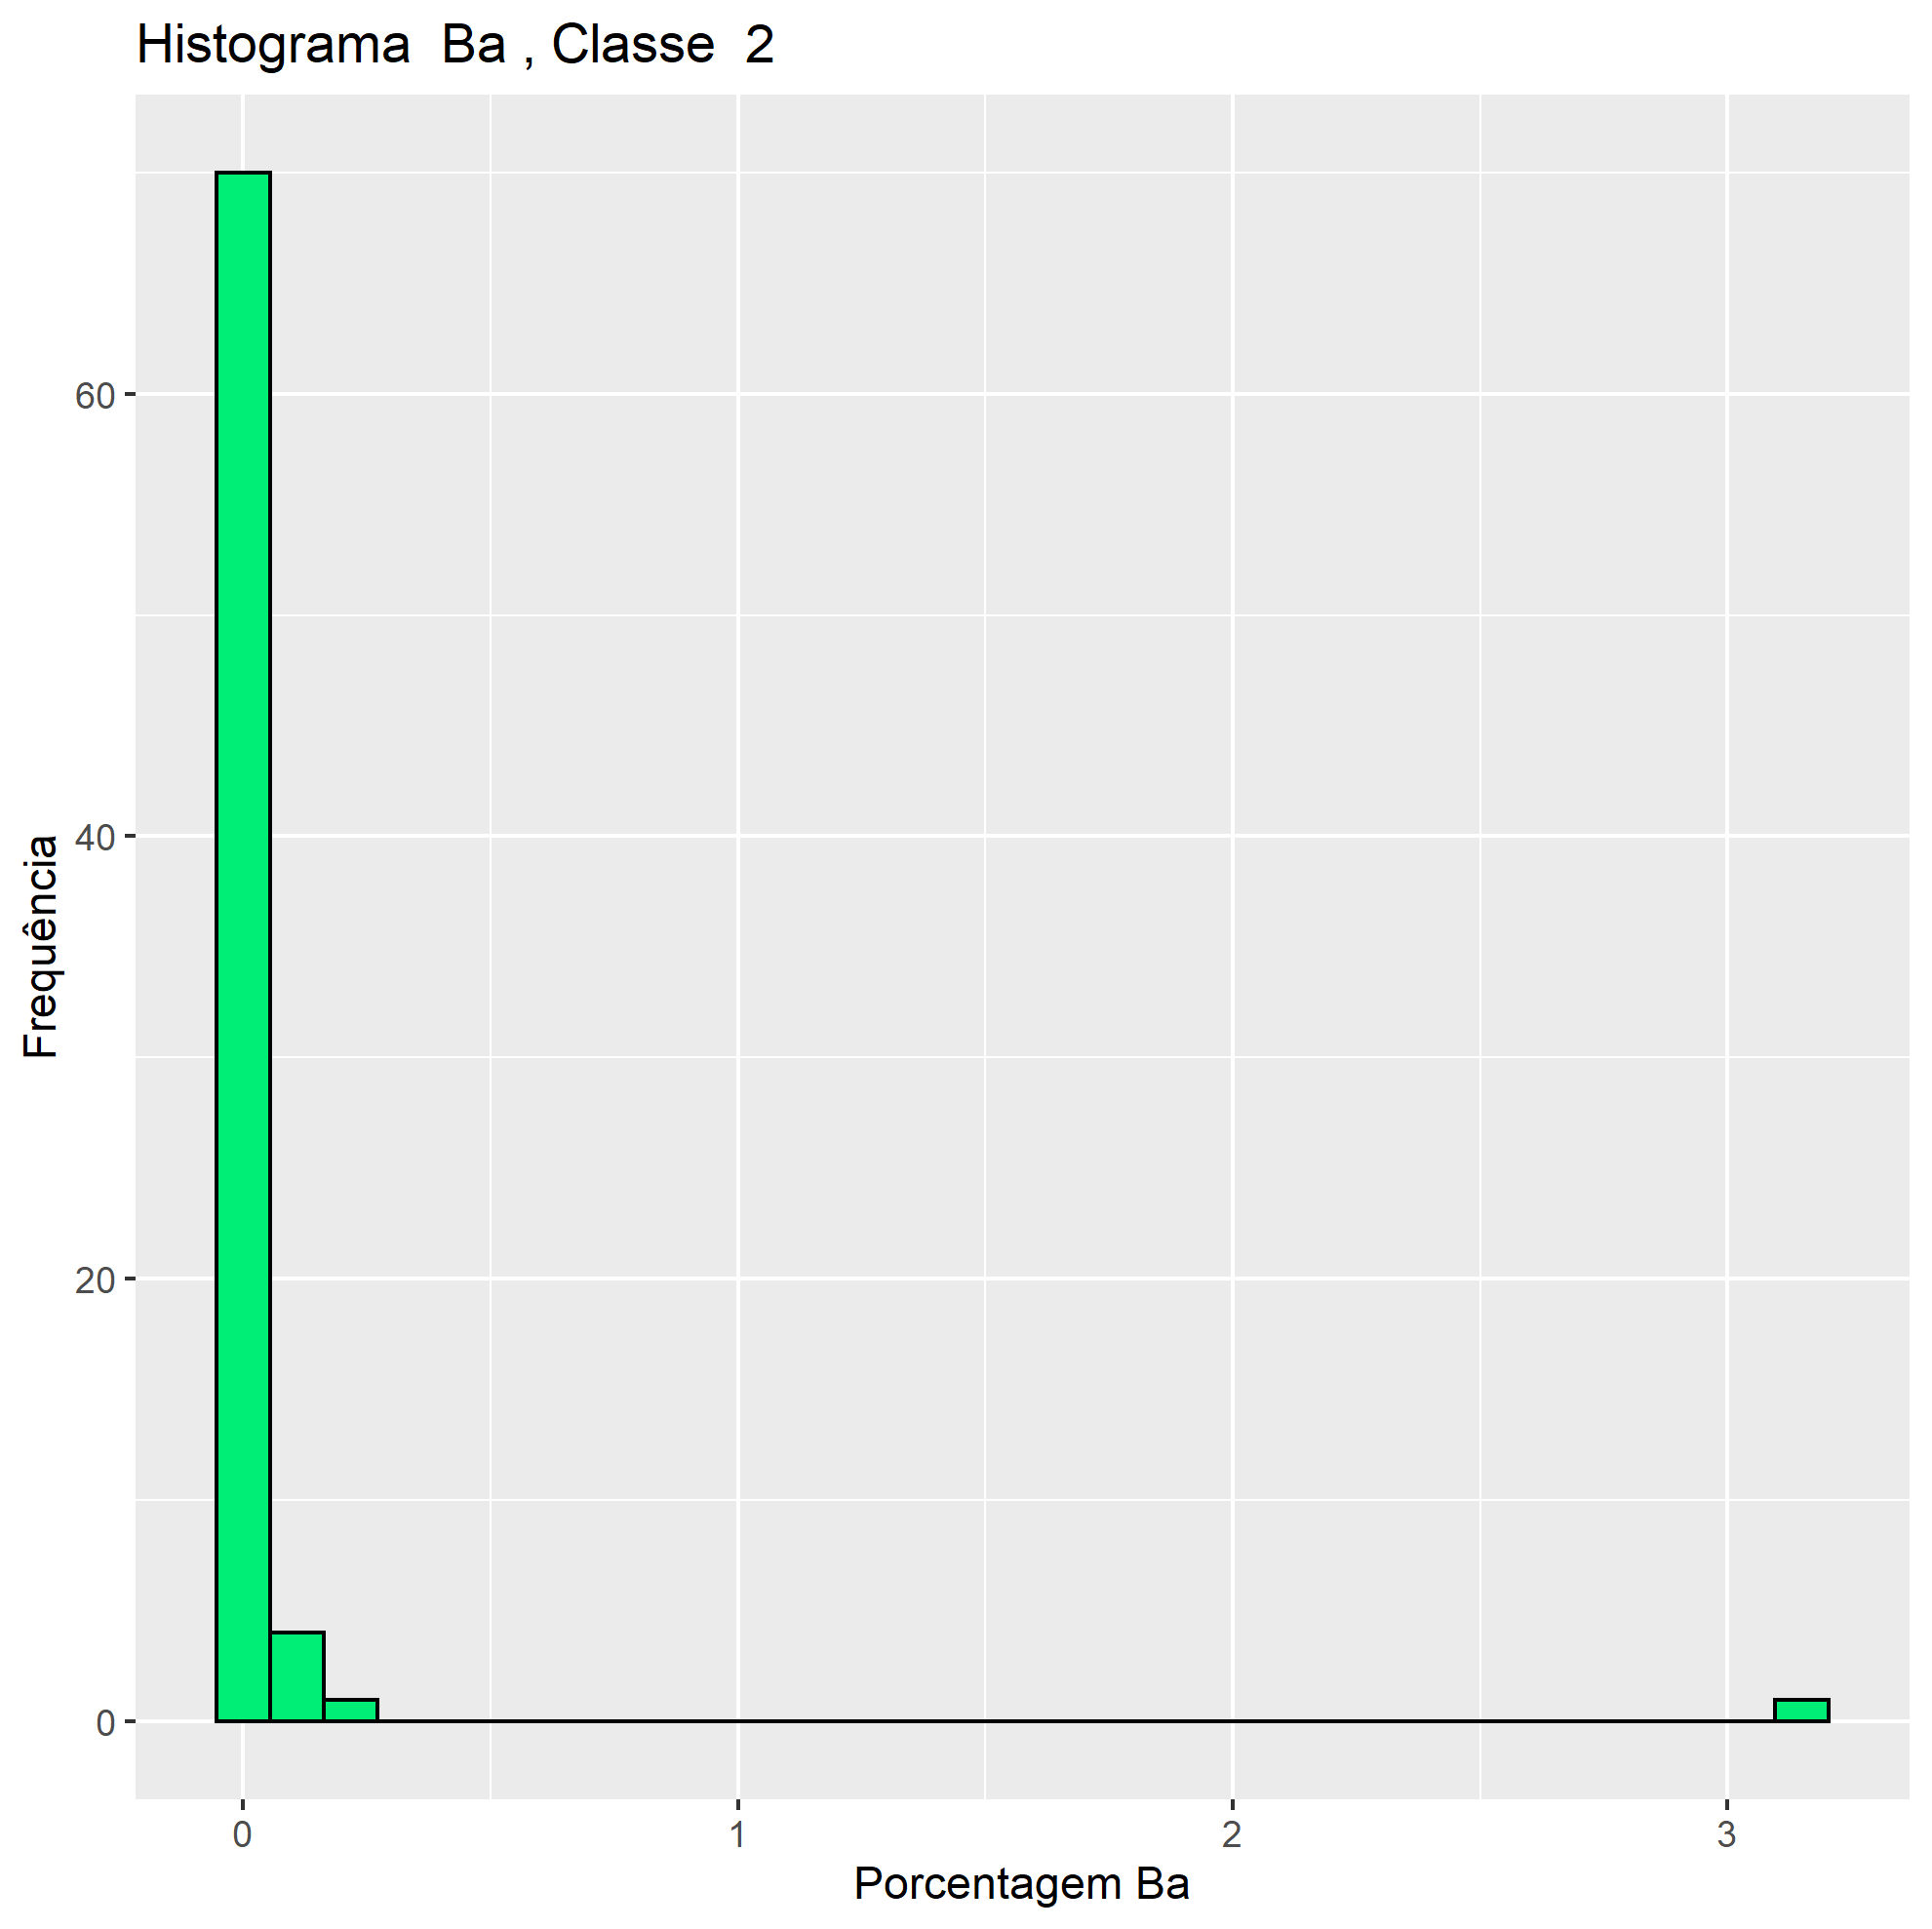
\includegraphics[width=5cm]{images/pt2/HistogramaBa_Classe2.png} % leia abaixo
\label{figura:histogramaal}
\end{figure}


\begin{figure}[h]
\caption{Histograma Mg - CLasse 2}
\centering % para centralizarmos a figura
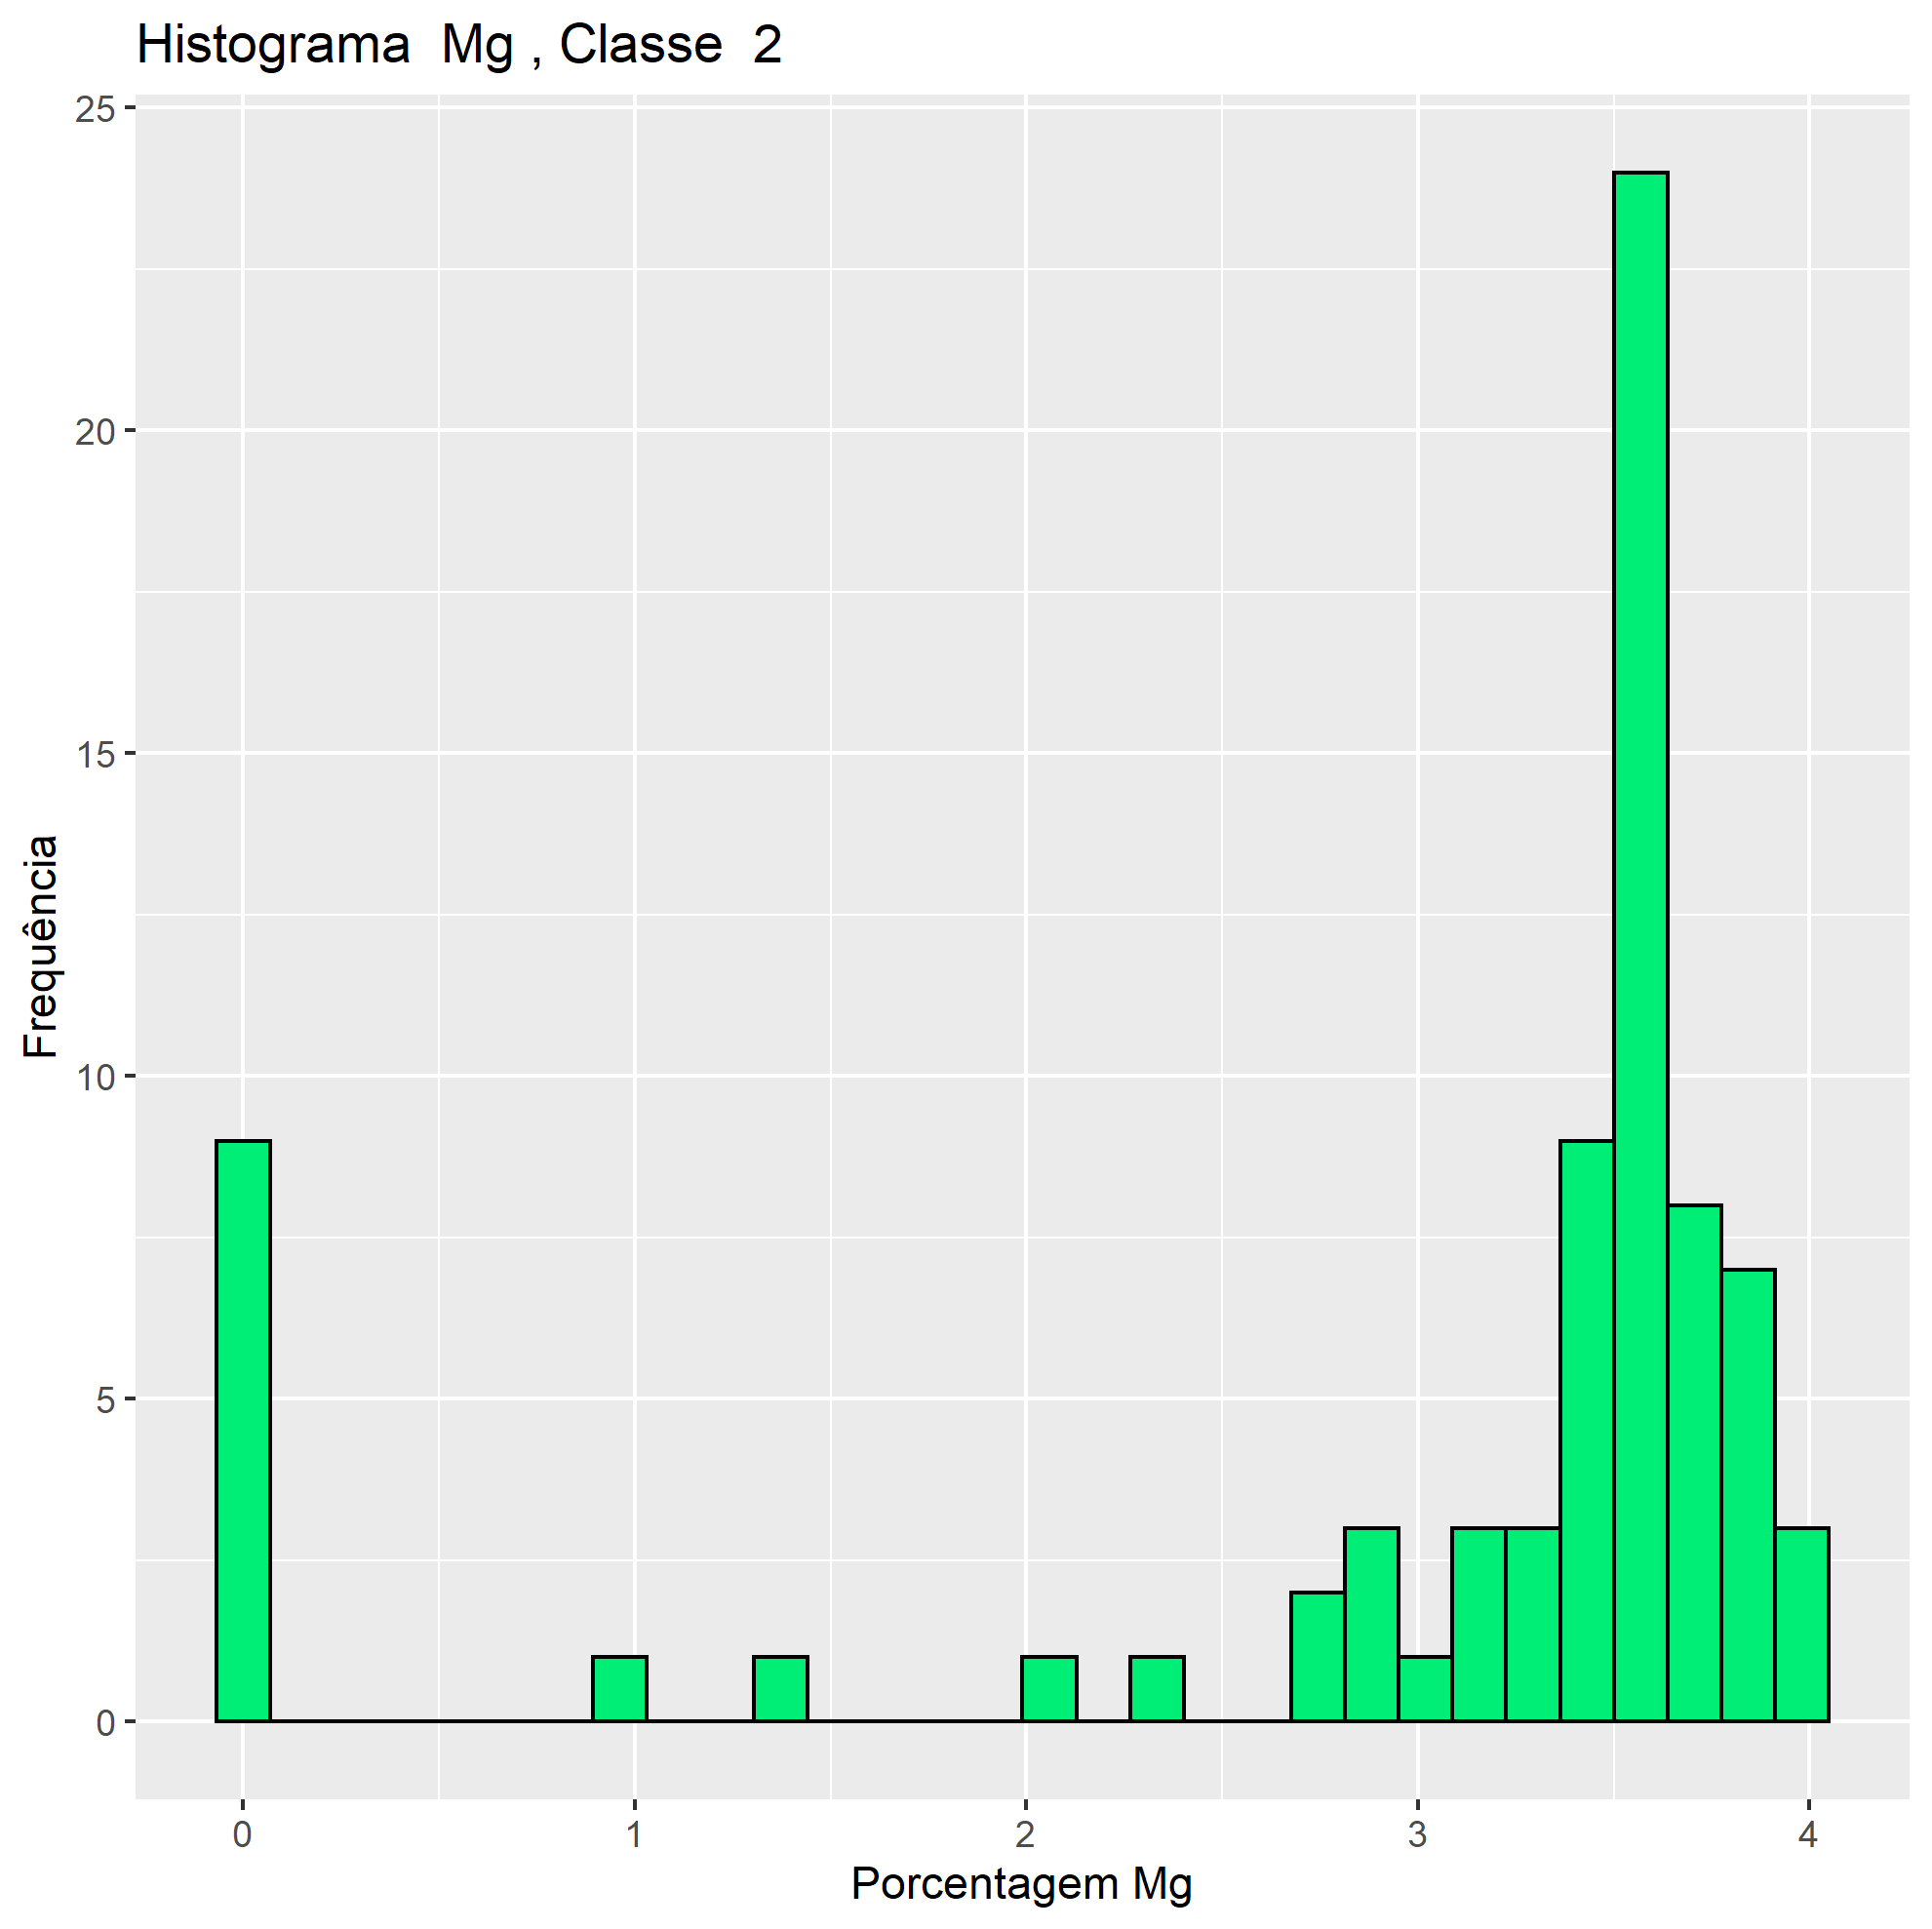
\includegraphics[width=5cm]{images/pt2/HistogramaMg_Classe2.png} % leia abaixo
\label{figura:histogramaal}
\end{figure}


\newpage %% ou \clearpage
\section{Imagens de Referência - Questão 3}

\begin{figure}[h]
\caption{Matriz de correlação mista}
\centering % para centralizarmos a figura
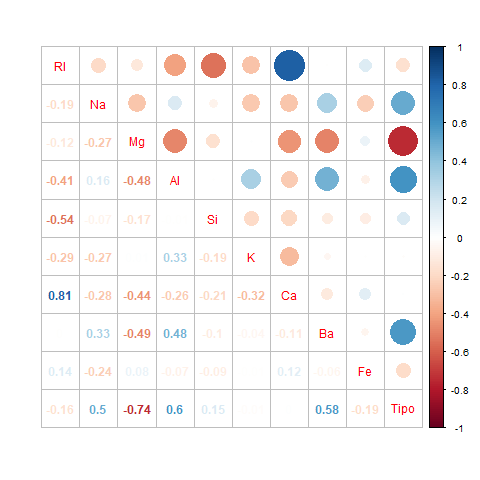
\includegraphics[width=5cm]{images/pt3/Matriz_Correlacao_mixed.png} % leia abaixo
\label{figura:histogramaal}
\end{figure}


\begin{figure}[h]
\caption{Si vs Ri}
\centering % para centralizarmos a figura
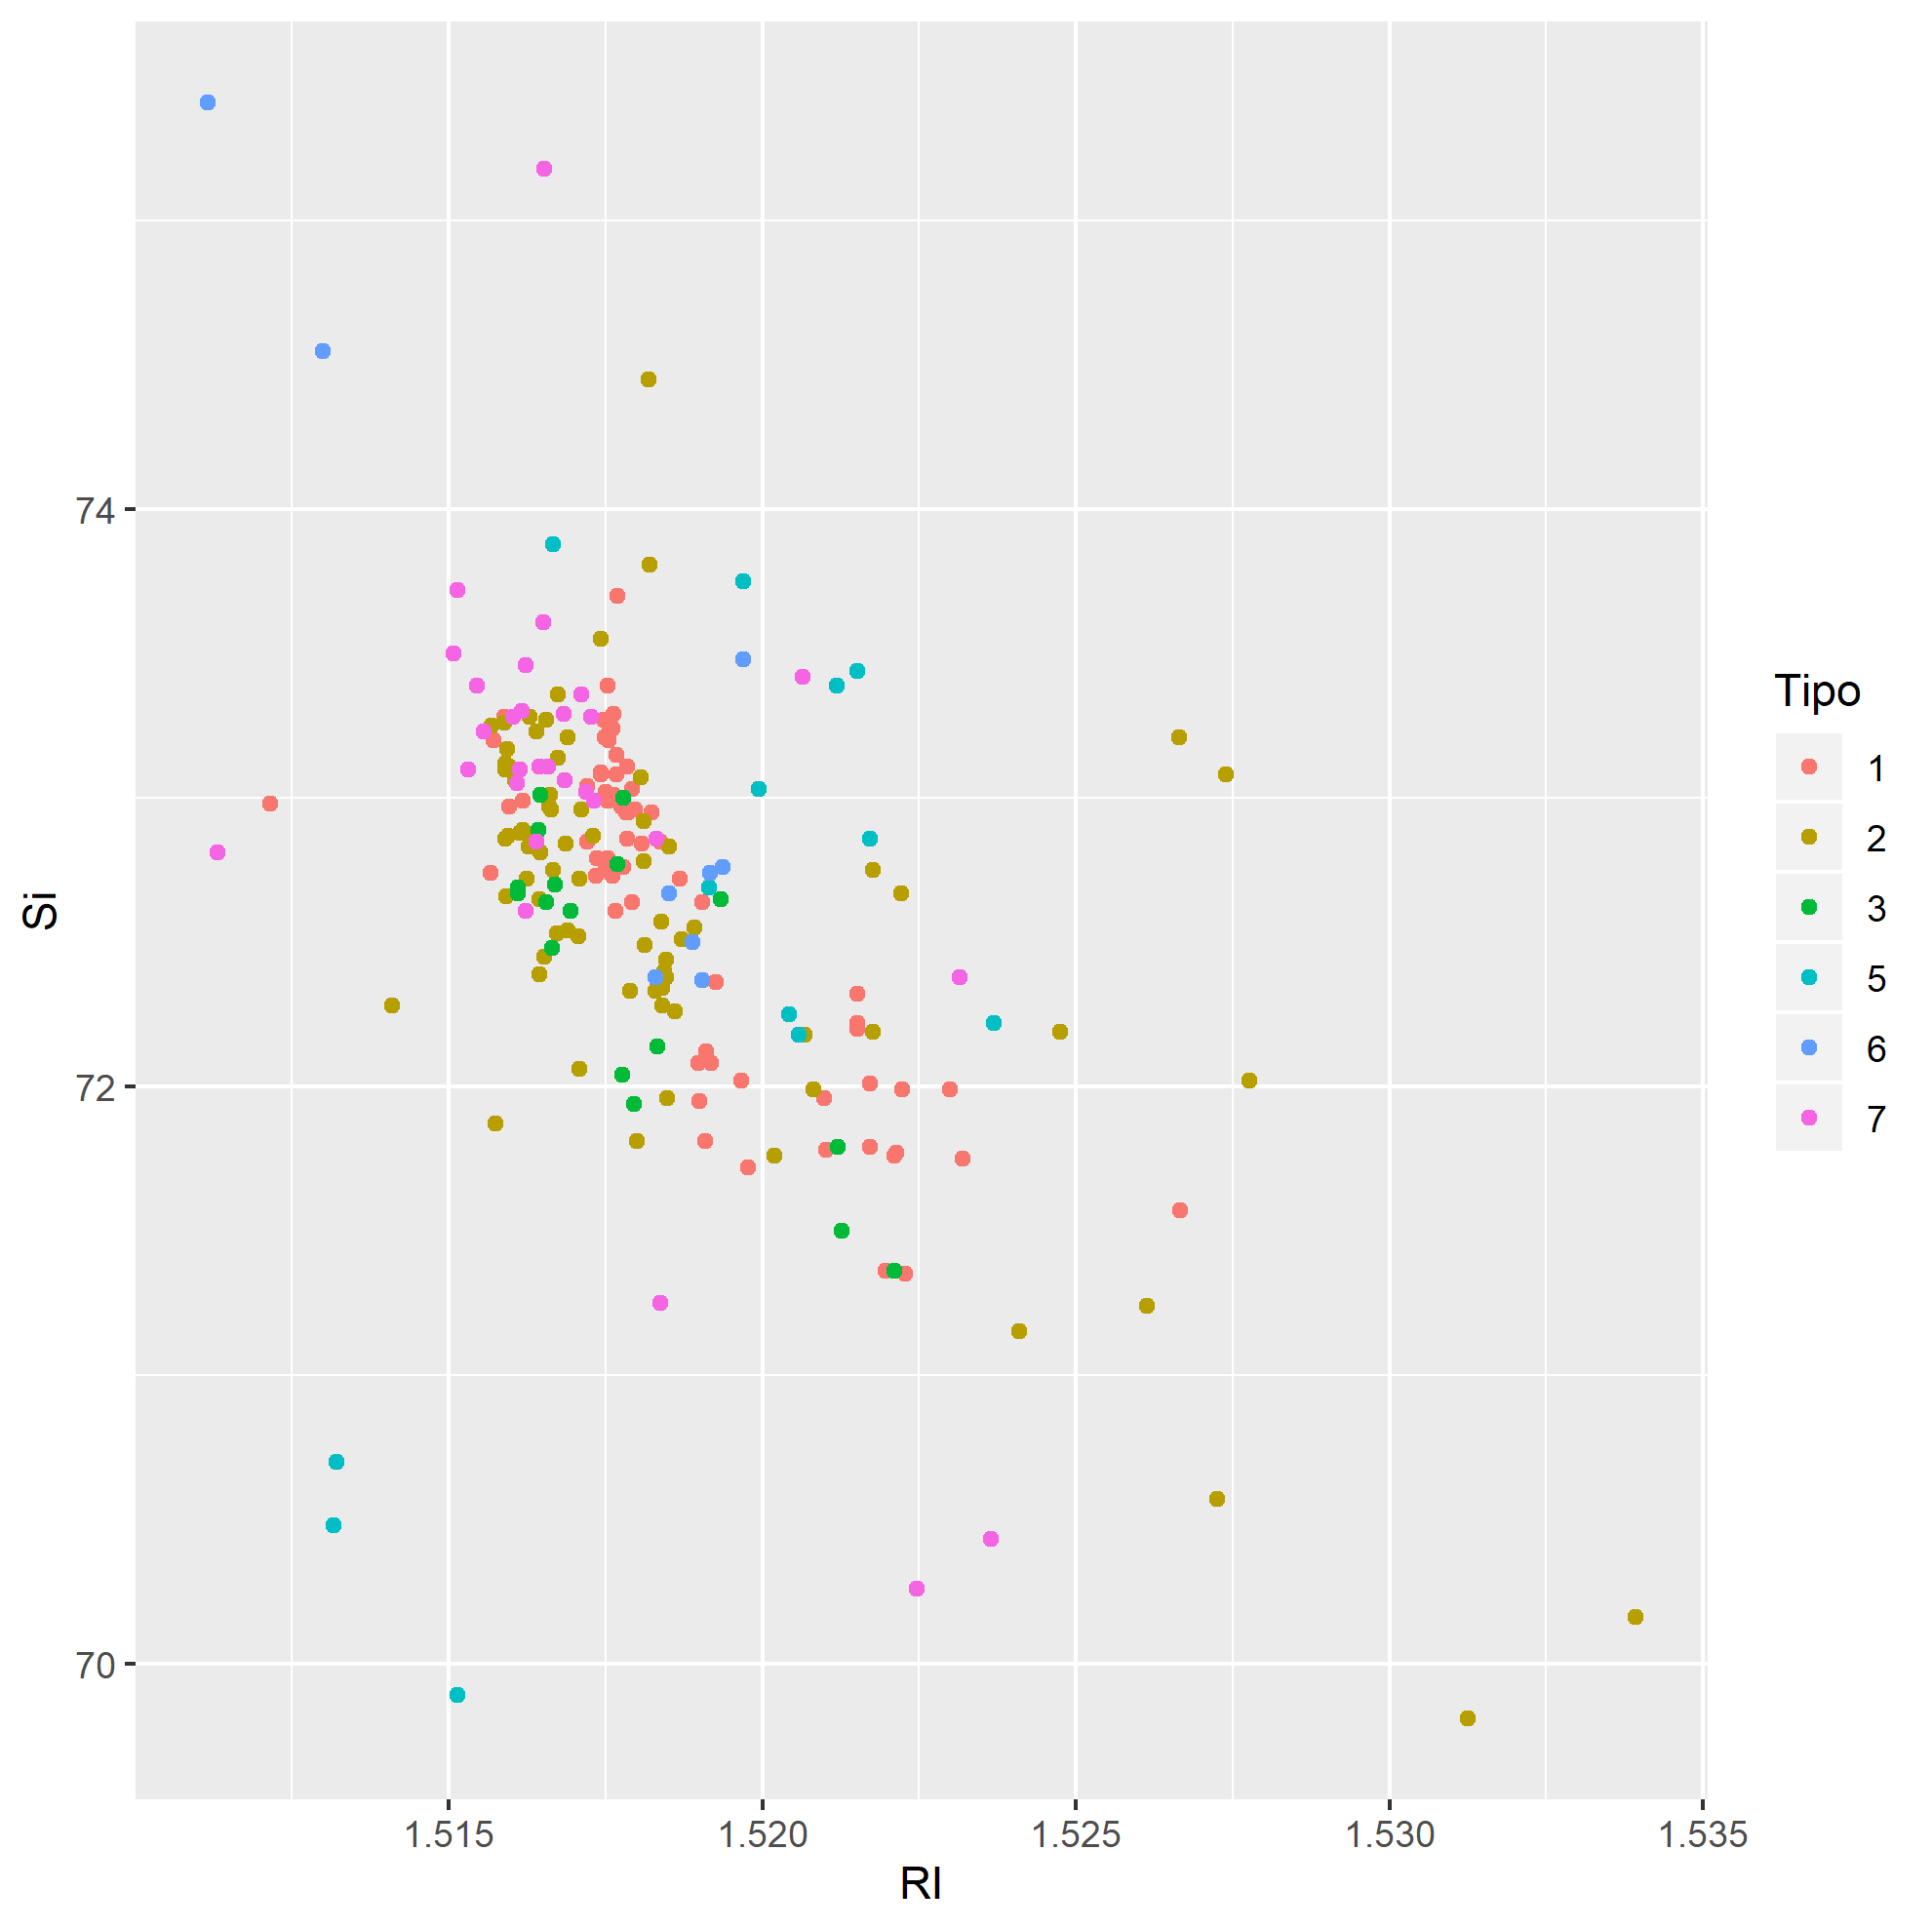
\includegraphics[width=5cm]{images/pt3/scatterplot_si_vs_ri.png} % leia abaixo
\label{figura:histogramaal}
\end{figure}


\begin{figure}[h]
\caption{Ca vs Ri}
\centering % para centralizarmos a figura
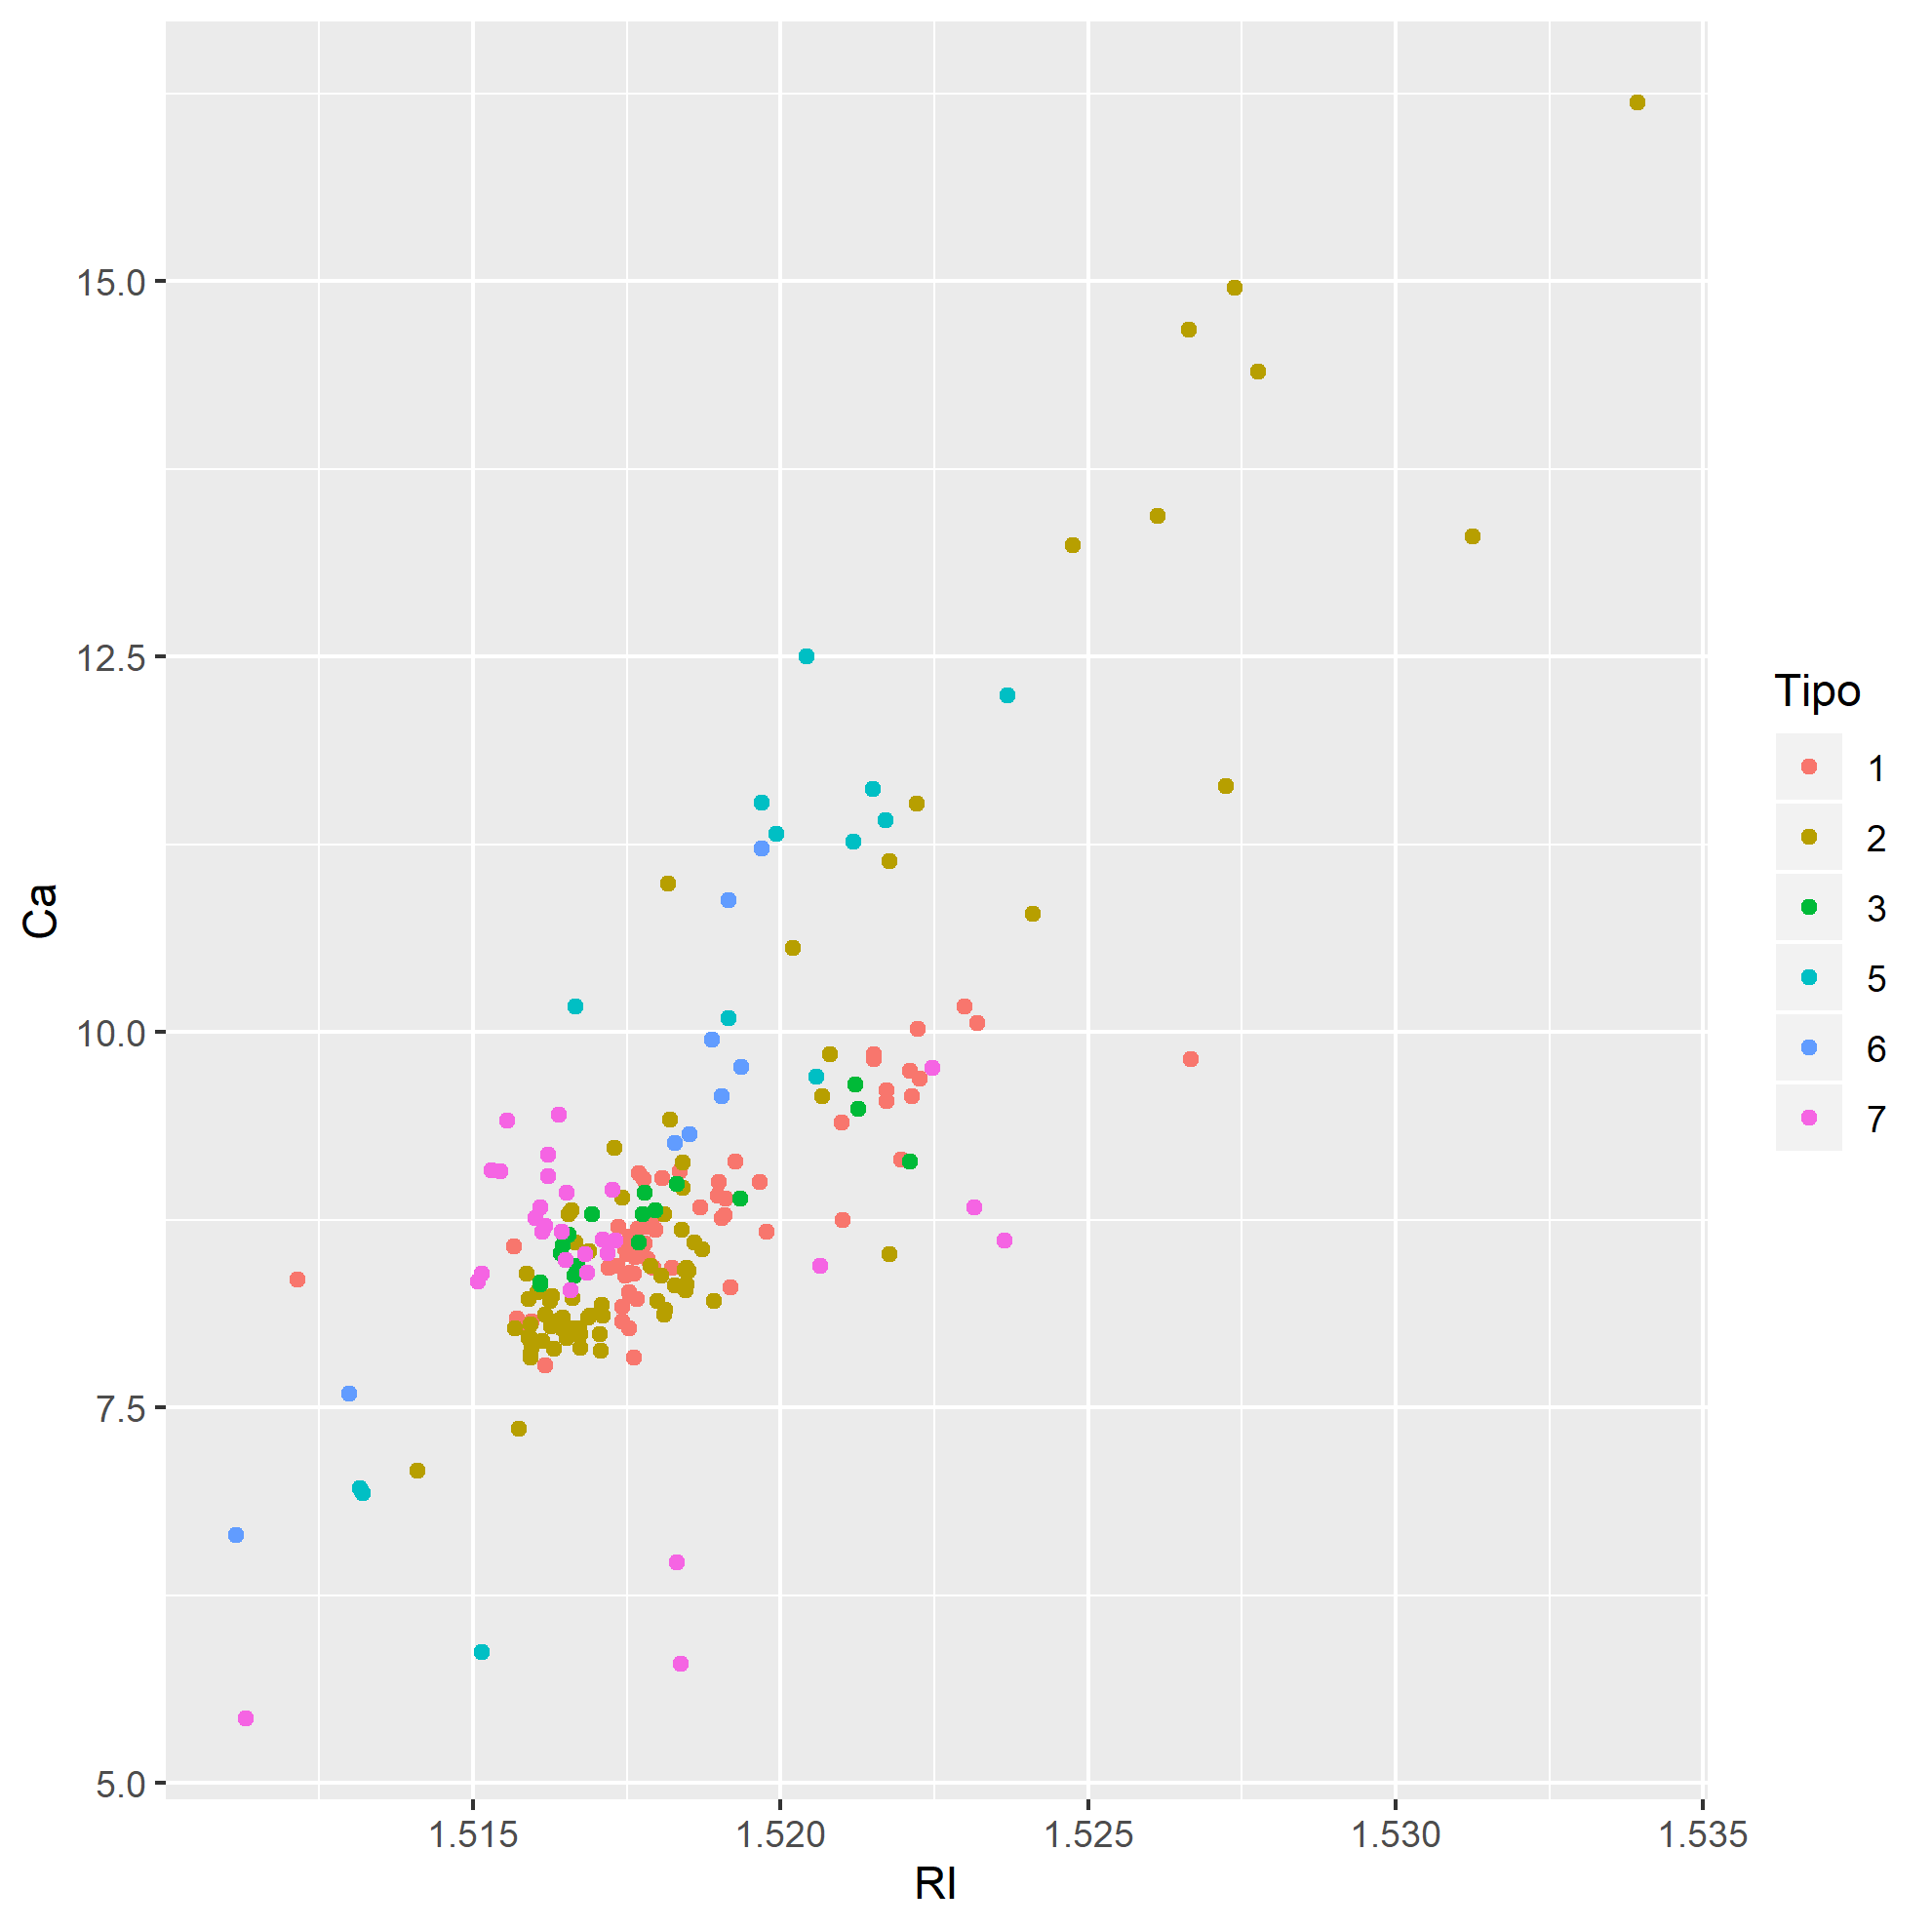
\includegraphics[width=5cm]{images/pt3/scatterplot_ca_vs_ri.png} % leia abaixo
\label{figura:histogramaal}
\end{figure}


\newpage %% ou \clearpage
\section{Imagens de Referência - Questão 4}

\begin{figure}[h]
\caption{PC1 vs PC1}
\centering % para centralizarmos a figura
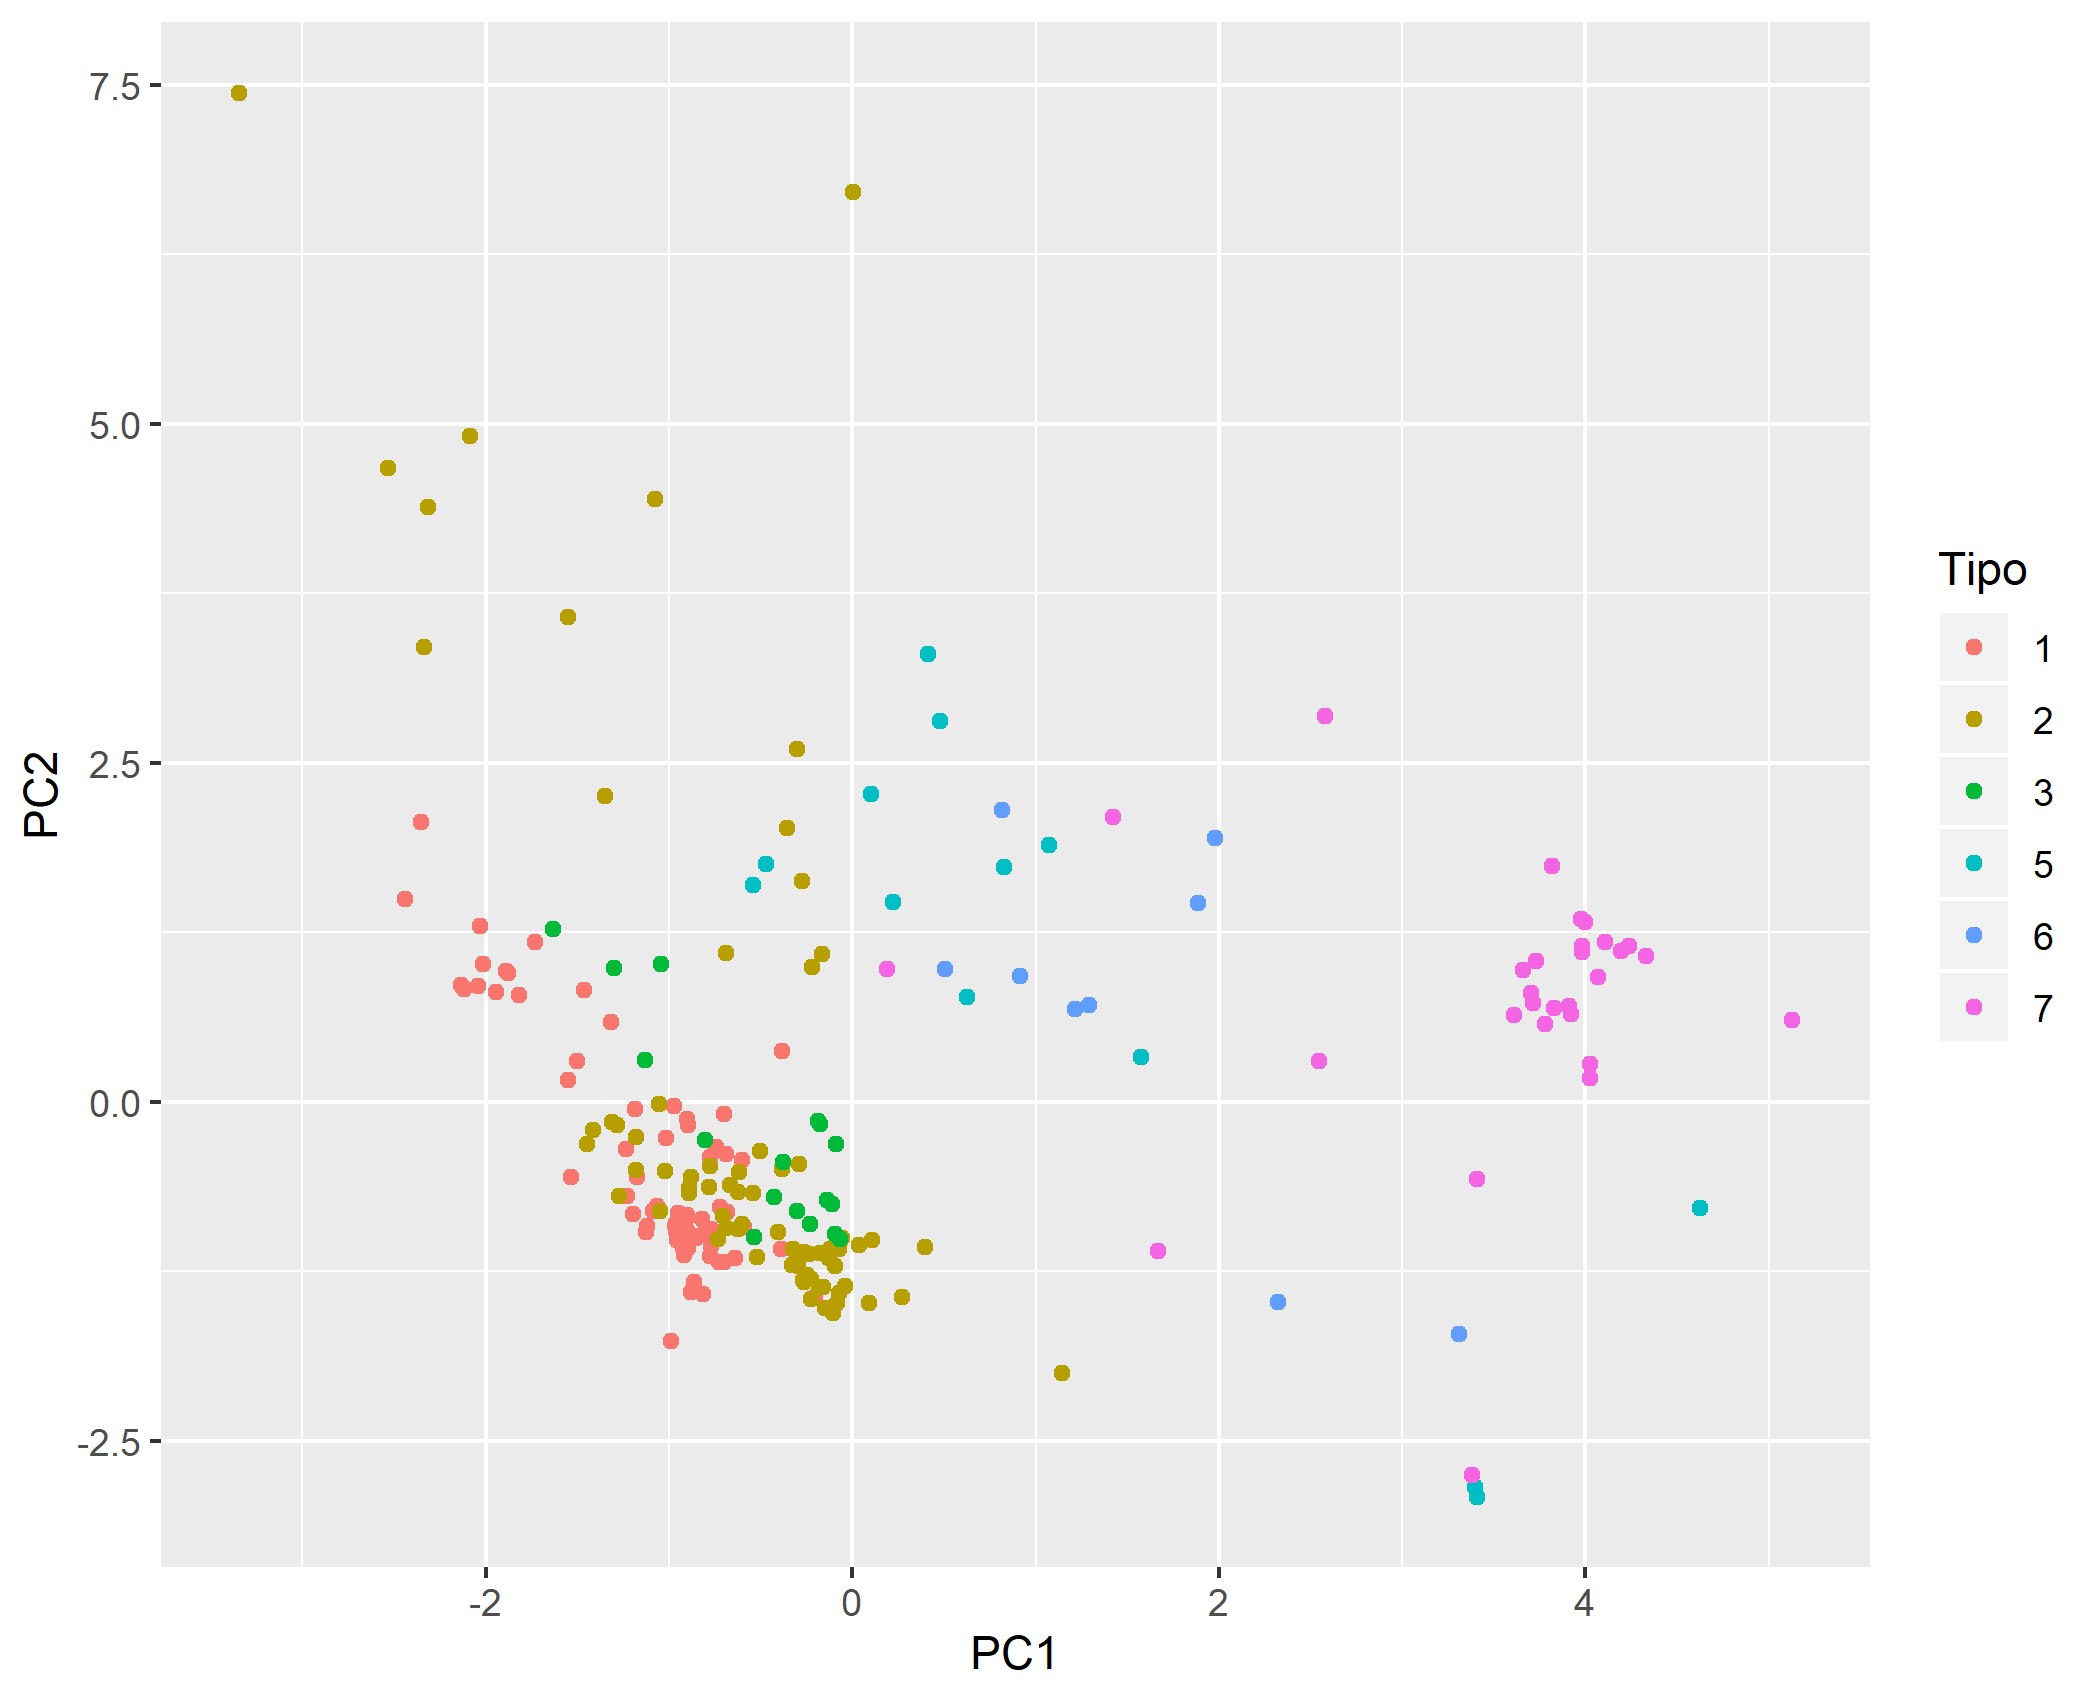
\includegraphics[width=5cm]{images/pt4/pc1vspc1.png} % leia abaixo
\label{figura:histogramaal}
\end{figure}

\begin{figure}[h]
\caption{Variâncias vs PCs}
\centering % para centralizarmos a figura
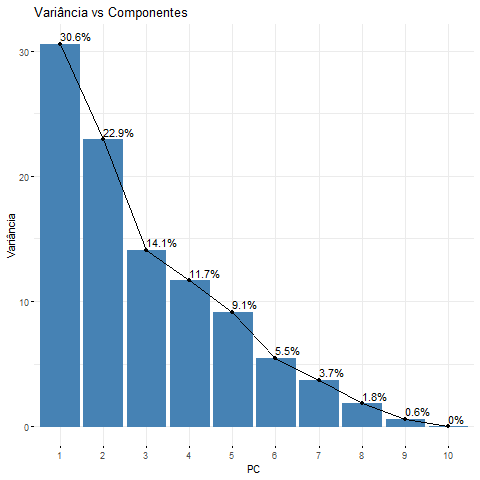
\includegraphics[width=5cm]{images/pt4/varianciavspcs.png} % leia abaixo
\label{figura:histogramaal}
\end{figure}
\end{document}